\documentclass{article}
\usepackage{graphicx}
\usepackage{caption}
\usepackage{float}
\captionsetup{justification=raggedright,singlelinecheck=false}
\title{Assignment \#1: Linux Kernel Installation}
\author{Muhammad Shafeen (22P-9278)}
\date{}

\begin{document}

\maketitle


\section*{Step 1: System Update and Upgrade}
\begin{figure}[H]
    \centering
    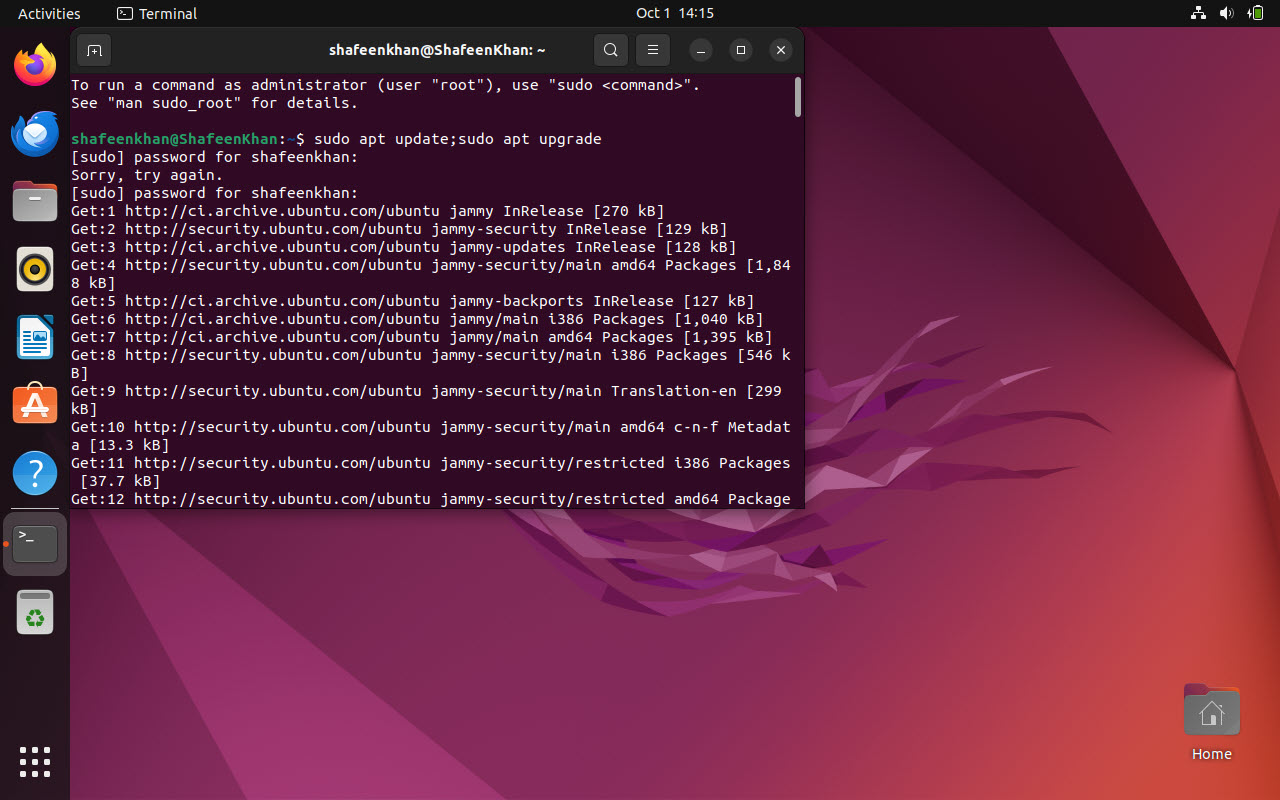
\includegraphics[width=0.8\textwidth]{78.jpg}
    \caption{Updating and upgrading the system before kernel compilation.}
\end{figure}

Before starting the kernel installation process,  updating the system using `sudo apt update` and `sudo apt upgrade` to ensure all packages are up to date.

\section*{Step 2: Installing Build Dependencies}
\begin{figure}[H]
    \centering
    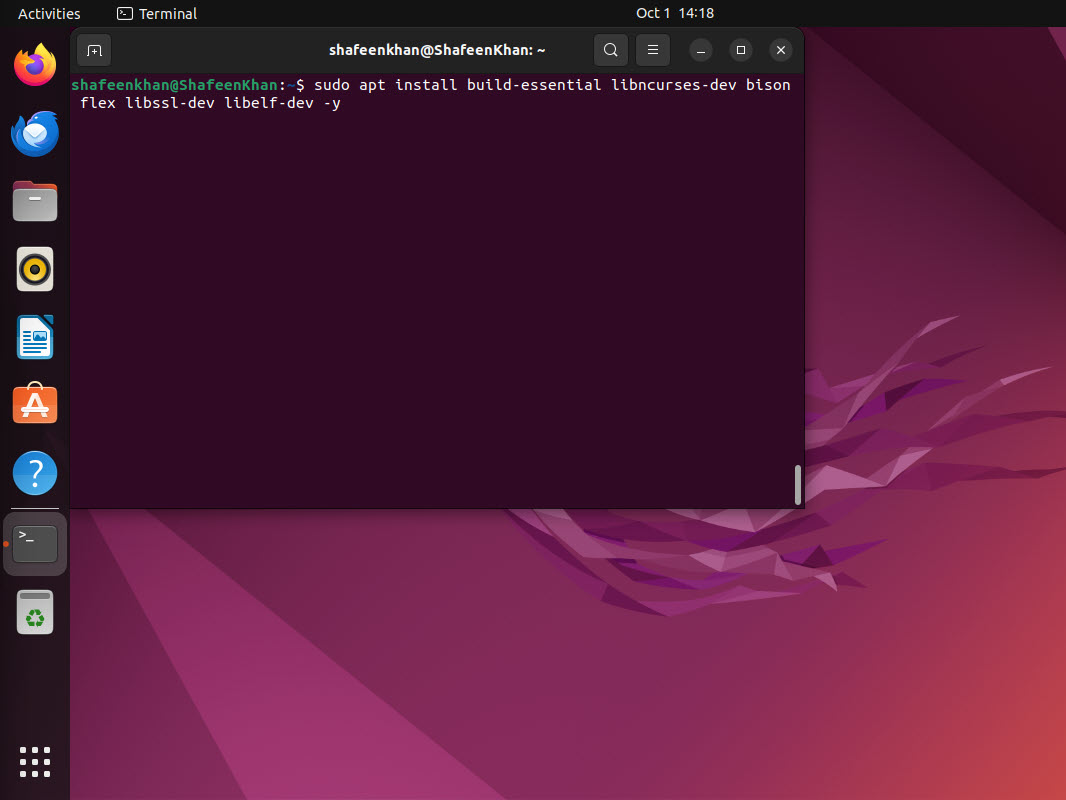
\includegraphics[width=0.8\textwidth]{76.jpg}
    \caption{Installing the required build dependencies for kernel compilation.}
\end{figure}

The user installs essential build tools like `build-essential`, `libncurses-dev`, `bison`, `flex`, and others required for compiling the Linux kernel.

\section*{Step 3: Verifying Installed Packages}
\begin{figure}[H]
    \centering
    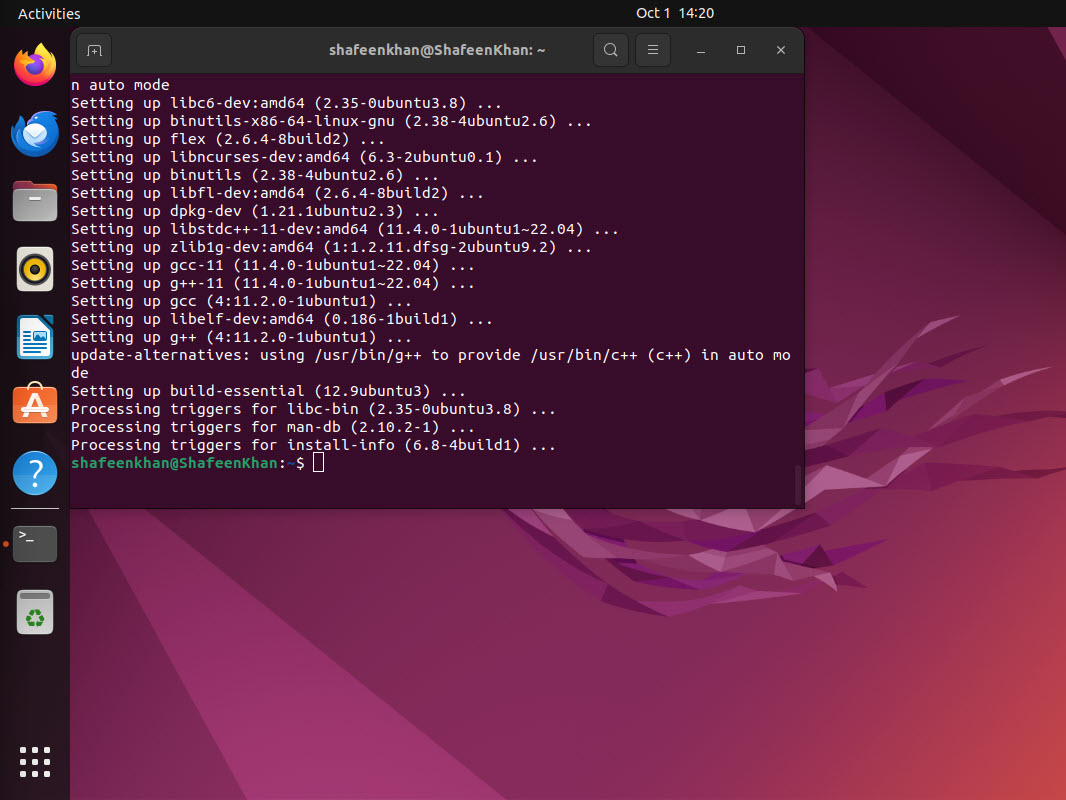
\includegraphics[width=0.8\textwidth]{75.jpg}
    \caption{Successful installation of required packages for kernel compilation.}
\end{figure}

% \section*{Step 4: Navigating to Kernel Build Directory}
% \begin{figure}[H]
%     \centering
%     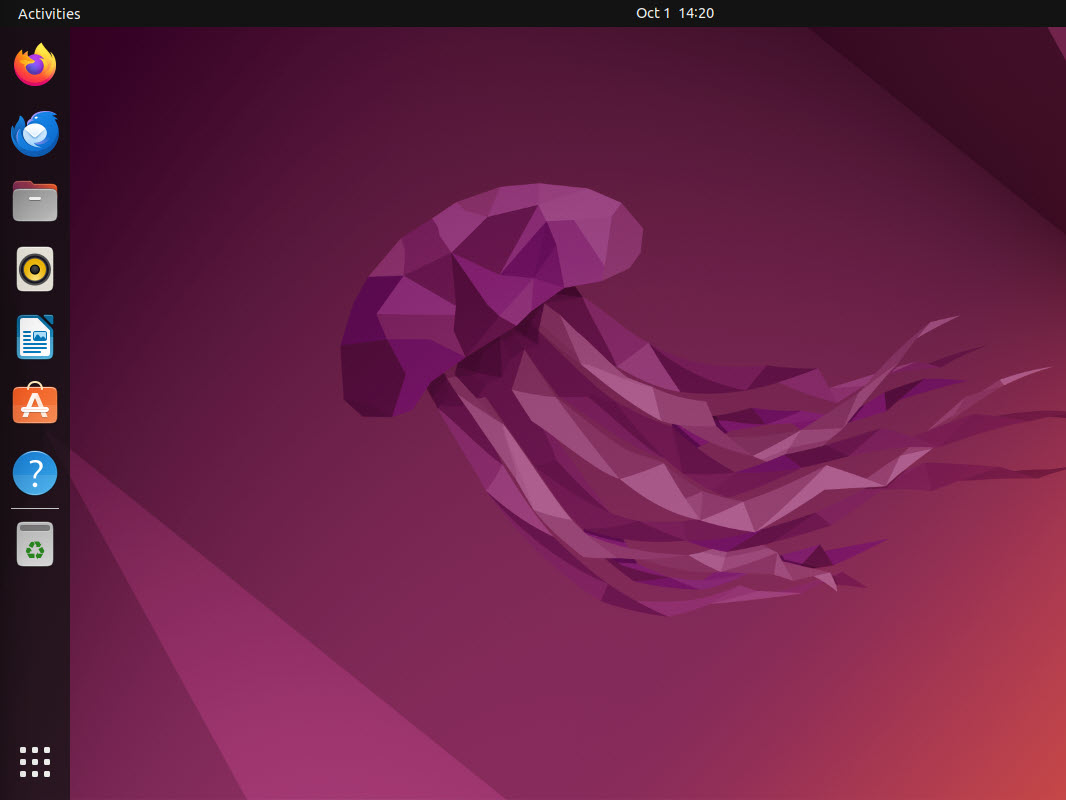
\includegraphics[width=0.8\textwidth]{74.jpg}
%     \caption{Creating a new directory for kernel build and downloading the kernel source.}
% \end{figure}


\section*{Step 4: Downloading Kernel \\ from Kernel Archives}
\begin{figure}[H]
    \centering
    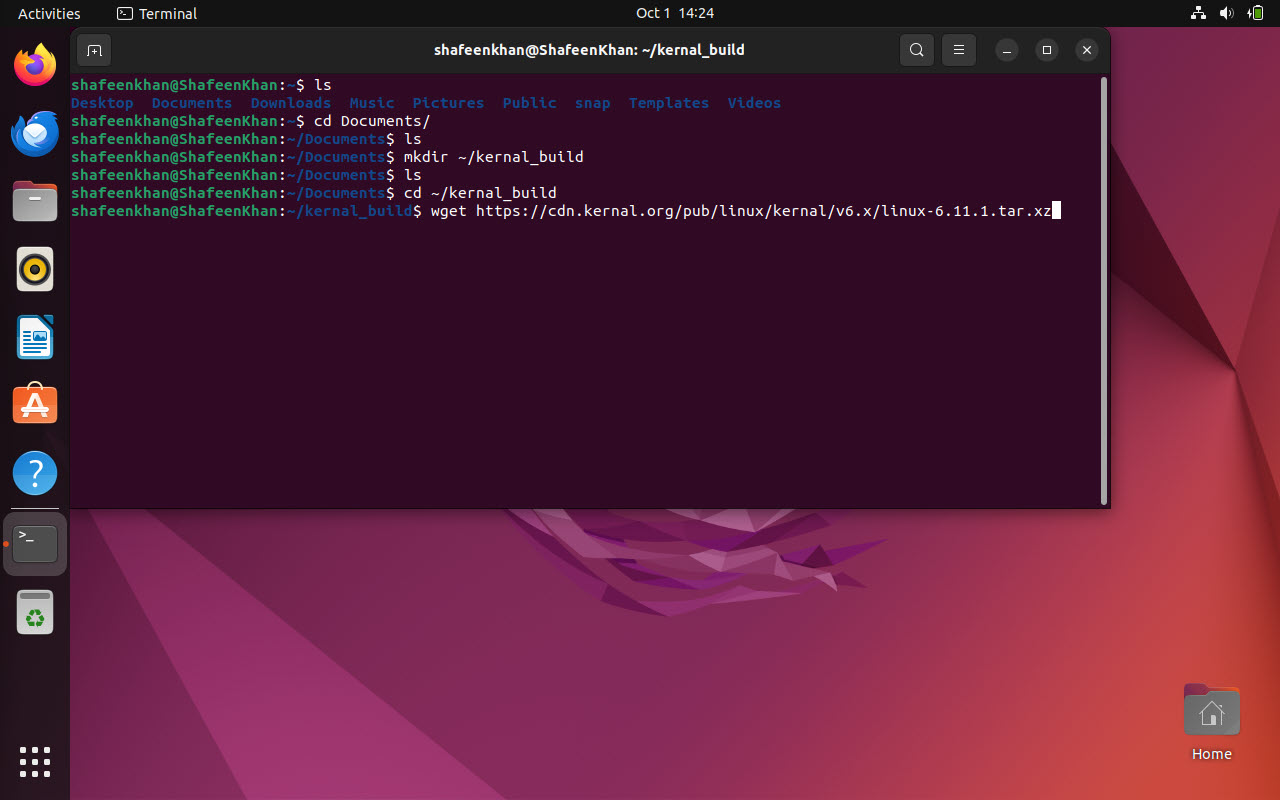
\includegraphics[width=0.8\textwidth]{73.jpg}
    \caption{Accessing the Linux Kernel Archives to download the latest stable version.}
\end{figure}


\section*{Step 5: Extracting the Kernel Source}
\begin{figure}[H]
    \centering
    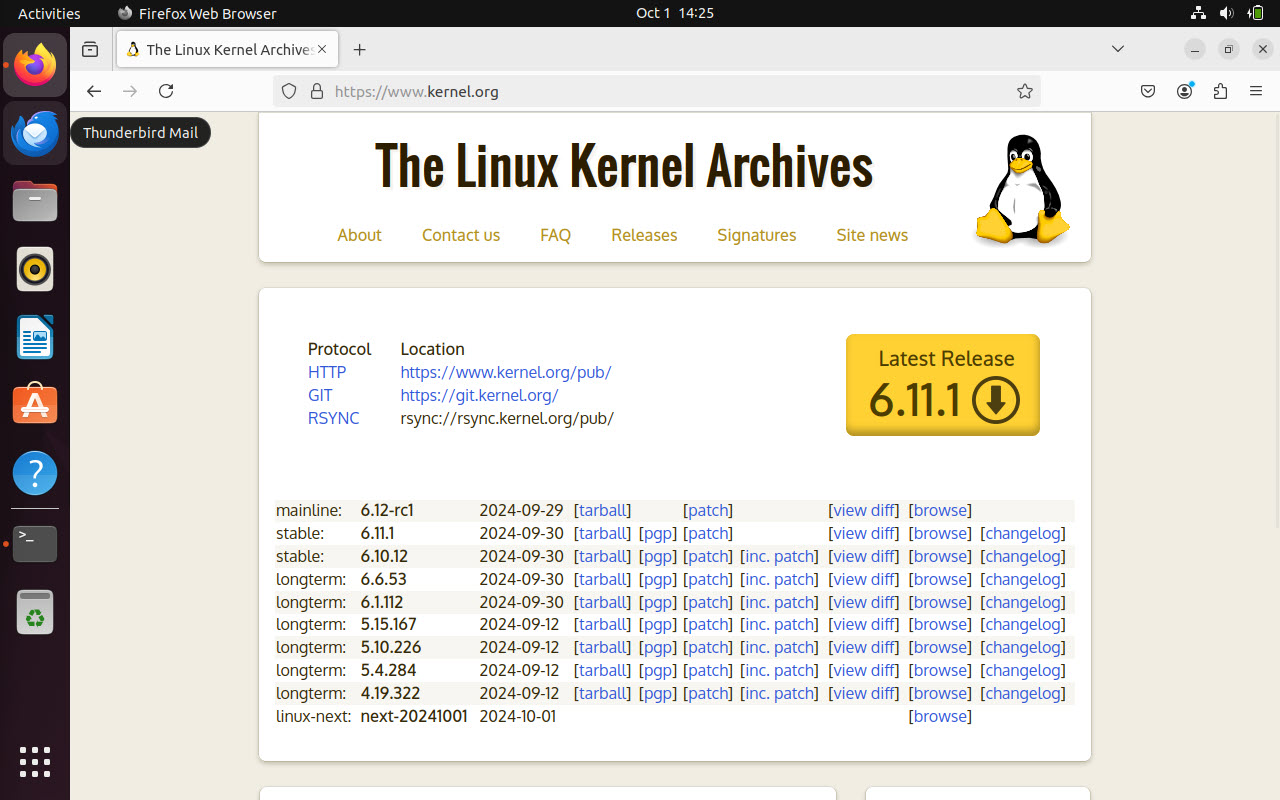
\includegraphics[width=0.8\textwidth]{72.jpg}
    \caption{Downloading the linux kernal}
\end{figure}
\begin{figure}[H]
    \centering
    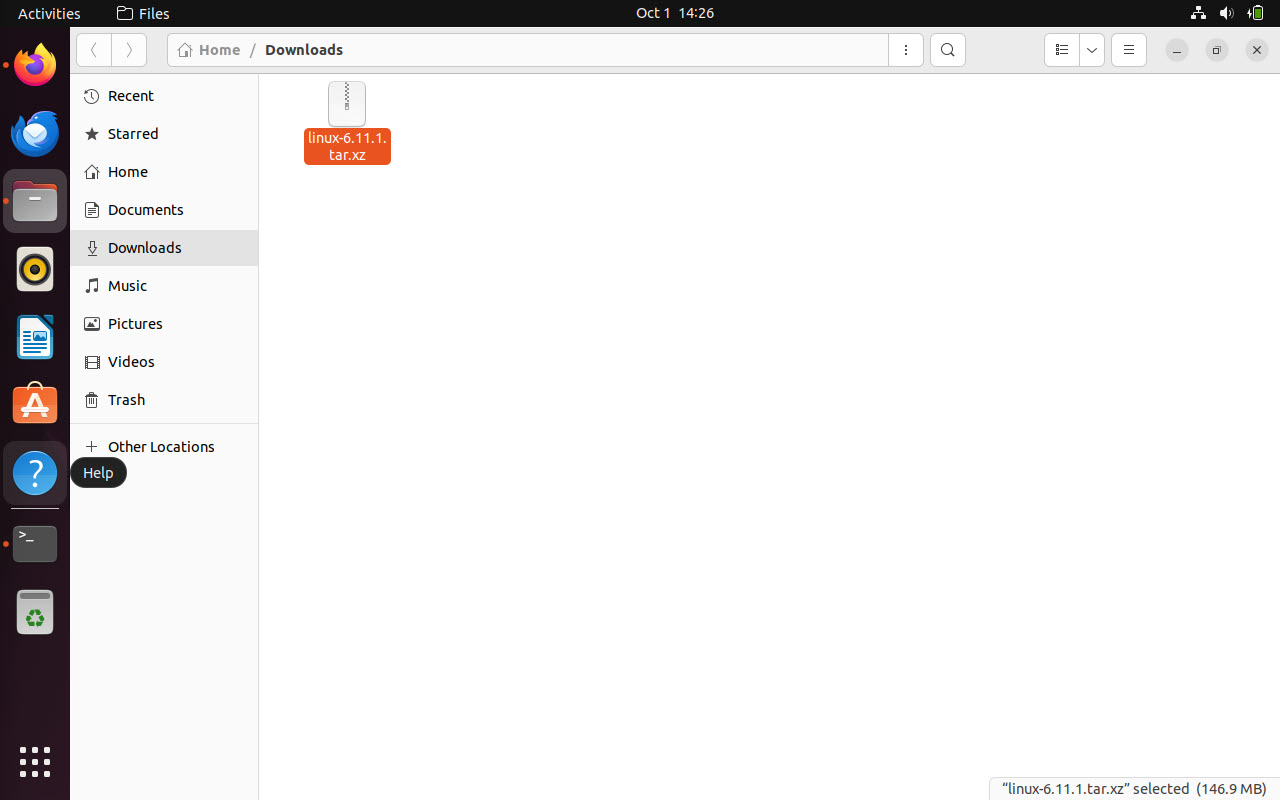
\includegraphics[width=0.8\textwidth]{71.jpg}
    \caption{Displaying the downloaded file}
\end{figure}

\section*{Step 6: Extract the linux source code file}
\begin{figure}[H]
    \centering
    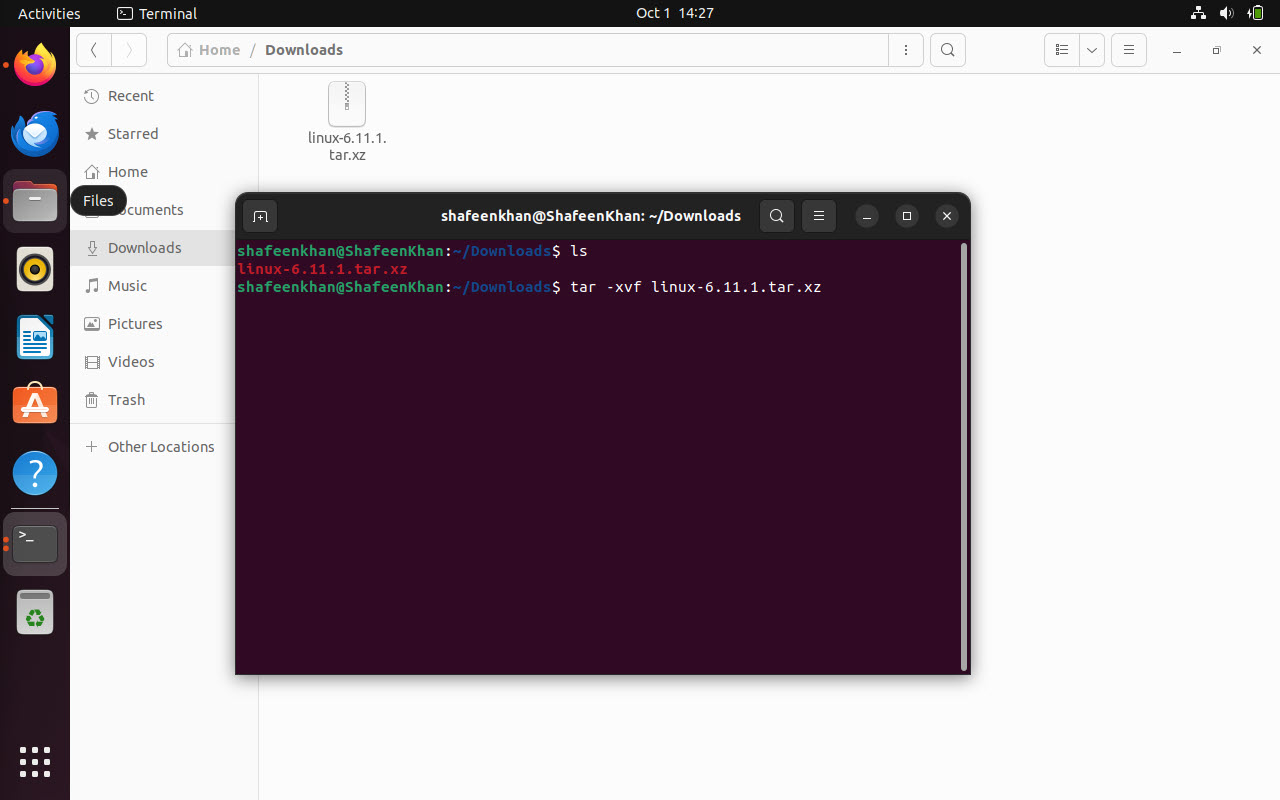
\includegraphics[width=0.8\textwidth]{70.jpg}
    \caption{Extracting the kernel source file using the `tar` command.}
\end{figure}

\begin{figure}[H]
    \centering
    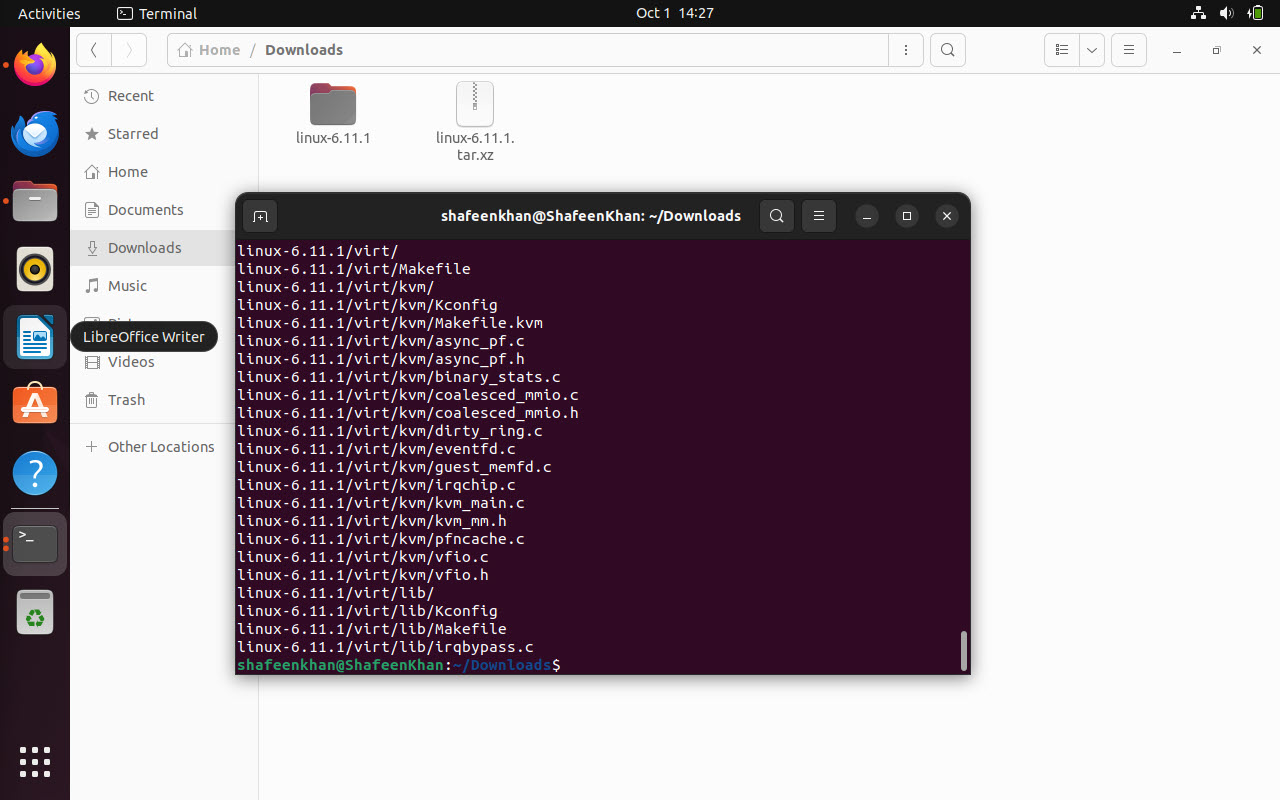
\includegraphics[width=0.8\textwidth]{69.jpg}
    \caption{Extraction completed}
\end{figure}


\section*{Step 7: Kernal Configuration}
\begin{figure}[H]
    \centering
    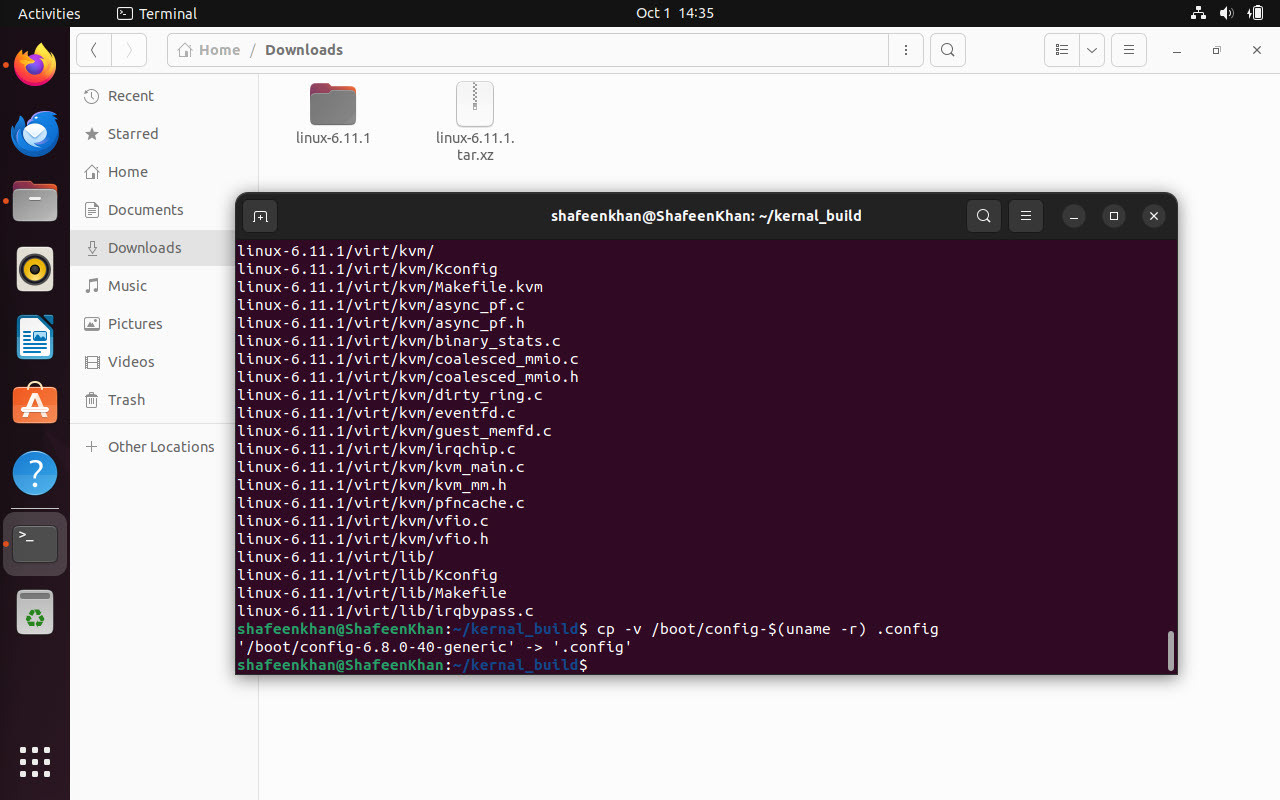
\includegraphics[width=0.8\textwidth]{65.jpg}
    \caption{Ensure similar configuration for new kernal}
\end{figure}
\subsection{Update Configuration Settings}
\begin{figure}[H]
    \centering
    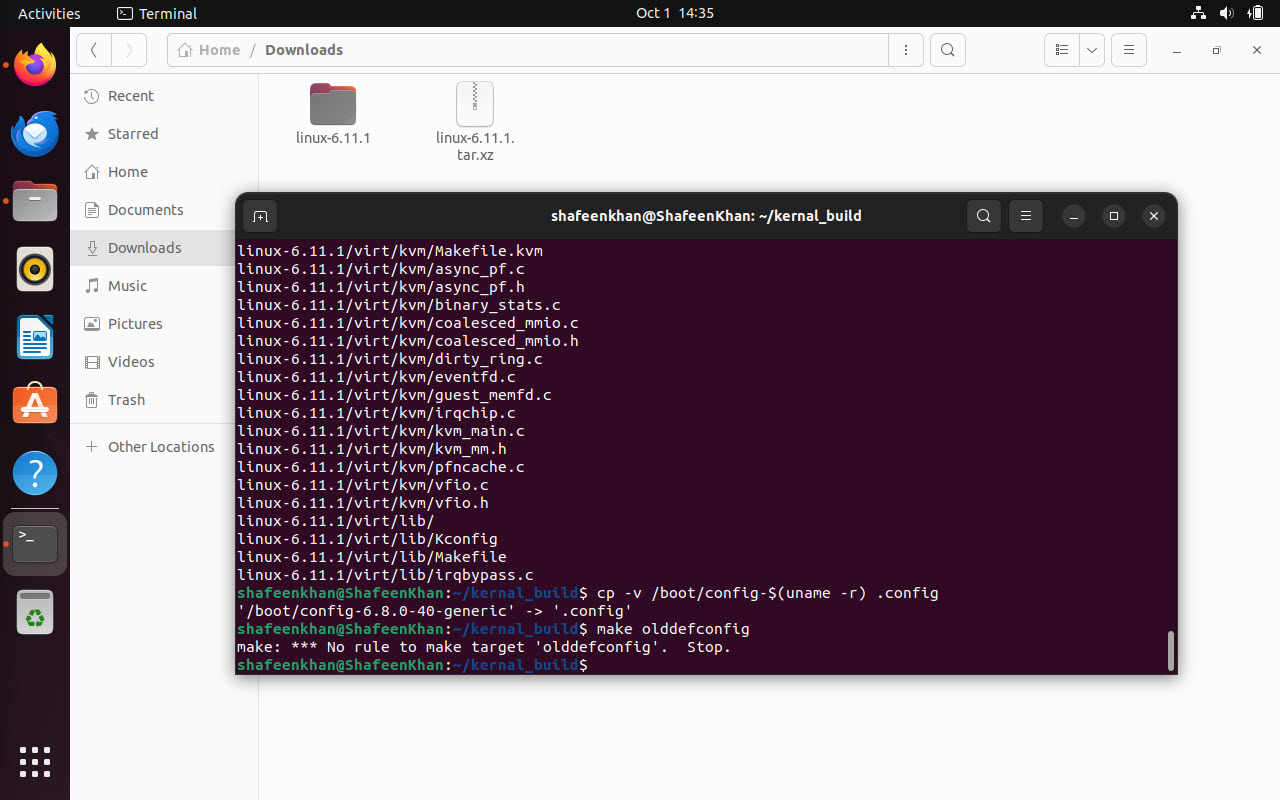
\includegraphics[width=0.8\textwidth]{64.jpg}
    \caption{This updates the copied configuration to be compatible with the new kernel version}
\end{figure}
\begin{figure}[H]
    \centering
    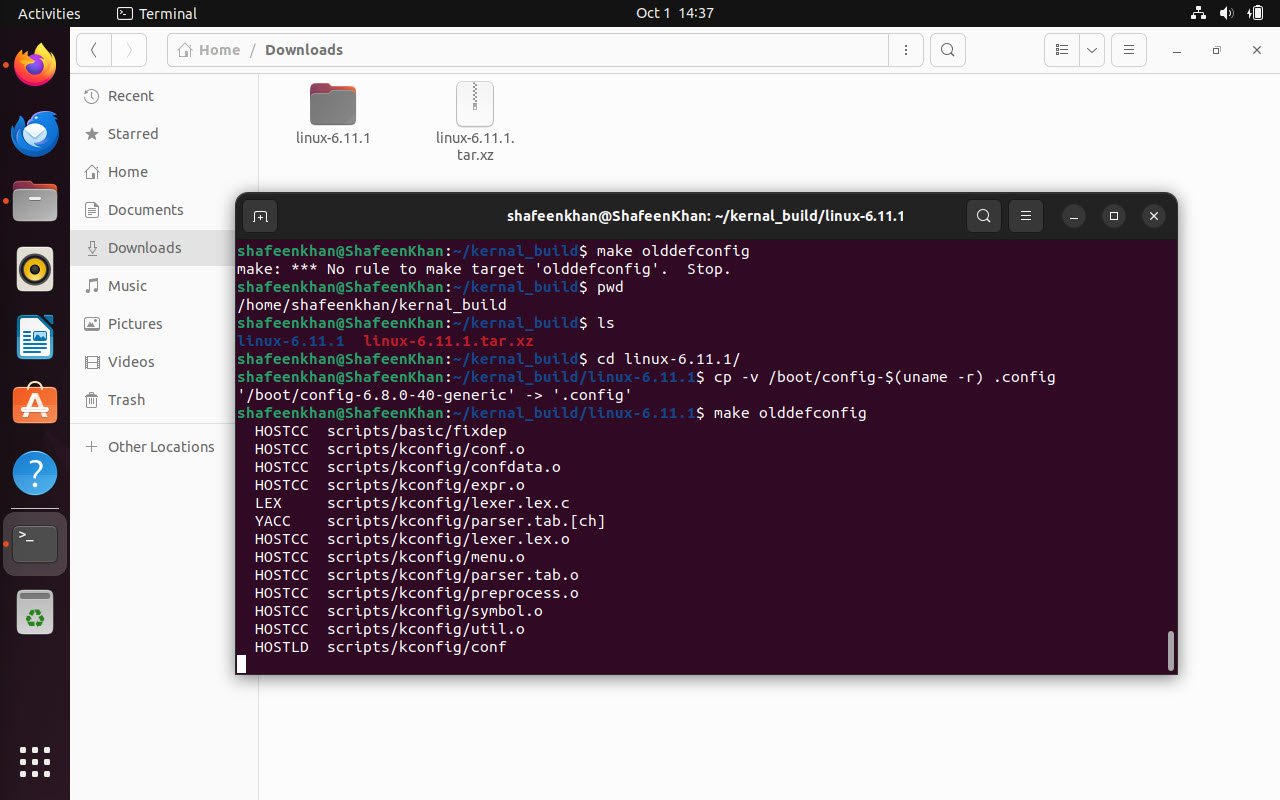
\includegraphics[width=0.8\textwidth]{63.jpg}
    \caption{In process}
\end{figure}

\subsection{Custom Kernal Configuration}
\begin{figure}[H]
    \centering
    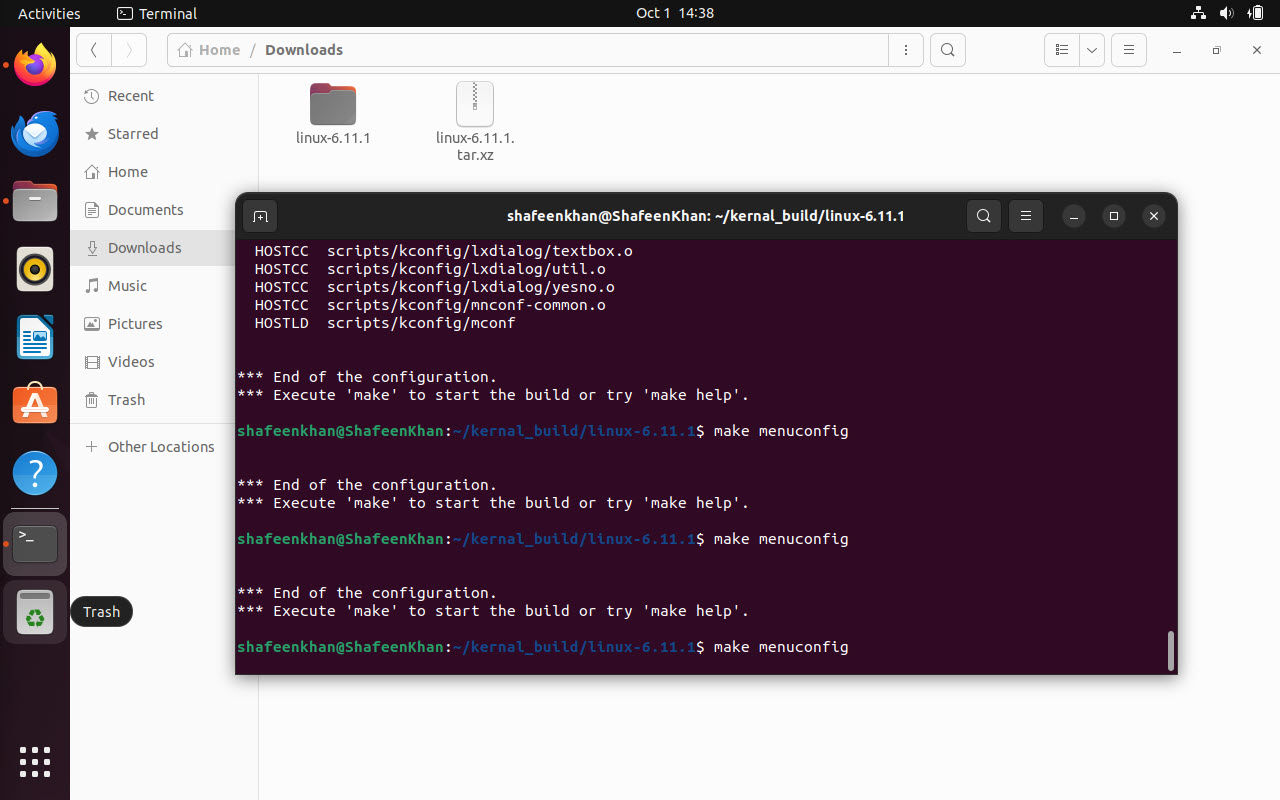
\includegraphics[width=0.8\linewidth]{62.jpg}
    \caption{This opens a text-based UI where you can navigate\\ and adjust kernel settings}
\end{figure}

\subsection{Bonus Challenge \\The UI - BASED interface \\for optional Tweaking }
\begin{figure}[H]
    \centering
    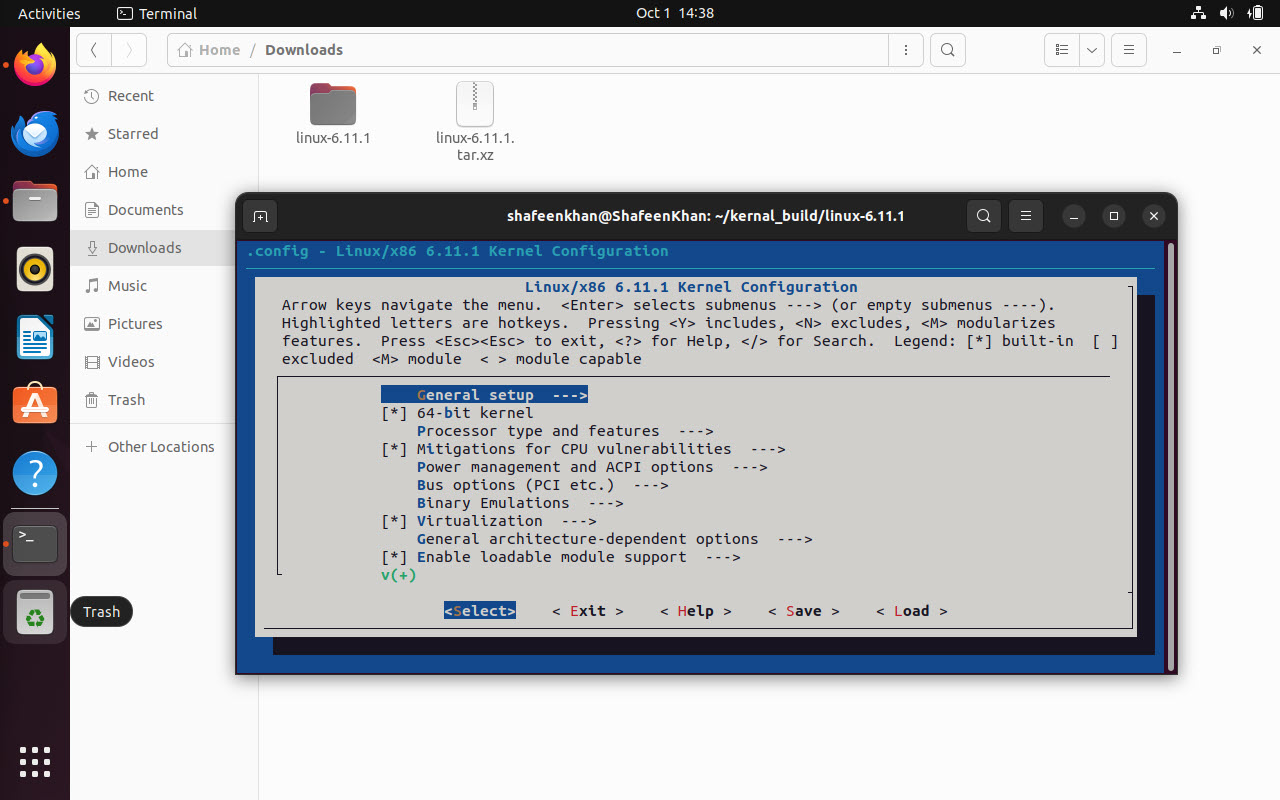
\includegraphics[width=0.8\linewidth]{61.jpg}
    \caption{The text-based UI where you can navigate\\ and adjust custom kernel settings for your benefit}
\end{figure}

\subsection{Kernel Configuration Setup \\- File System Options}
\begin{figure}[H]
    \centering
    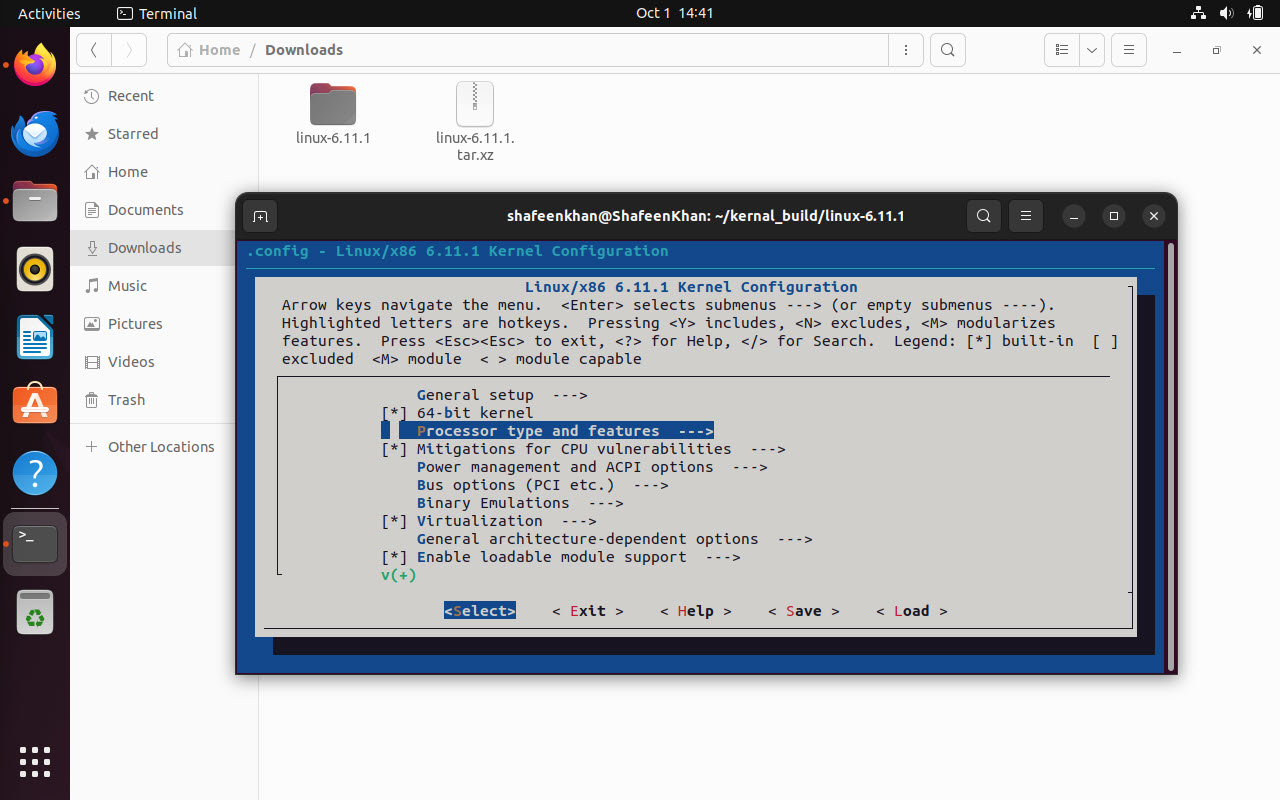
\includegraphics[width=0.8\linewidth]{60.jpg}
    \caption{Navigating the kernel configuration menu to modify the file system options. The user is in the kernel configuration interface for Linux version 6.11.1. Various subsystems, including networking support and device drivers, are shown with a focus on selecting file systems for tweaking.}
\end{figure}

\subsection{Kernel Configuration Setup\\ - General Setup}
\begin{figure}[H]
    \centering
    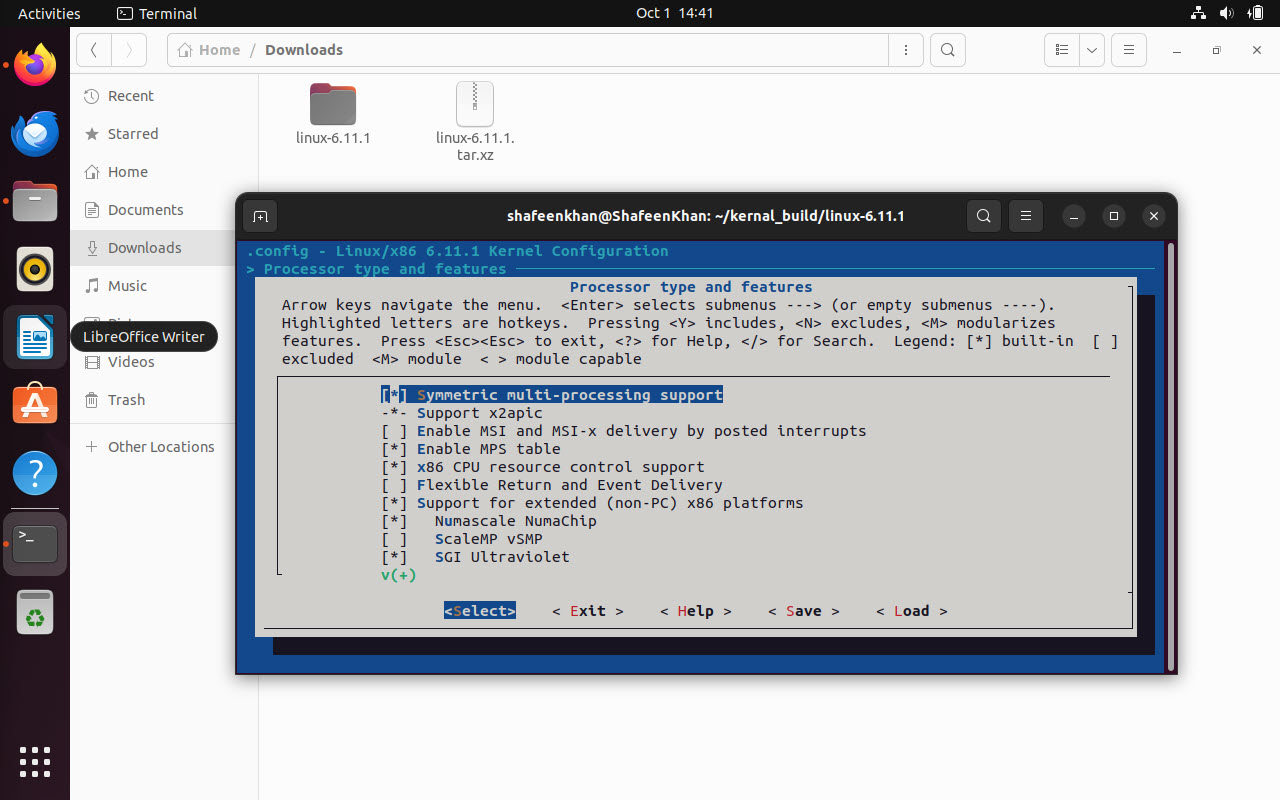
\includegraphics[width=0.8\linewidth]{59.jpg}
    \caption{Turning on the Symmetric multi-processing support for faster computations and to increase speed}
\end{figure}


\subsection{Kernel Configuration Setup\\ -  Optimizing for my own Specific Processor}
\begin{figure}[H]
    \centering
    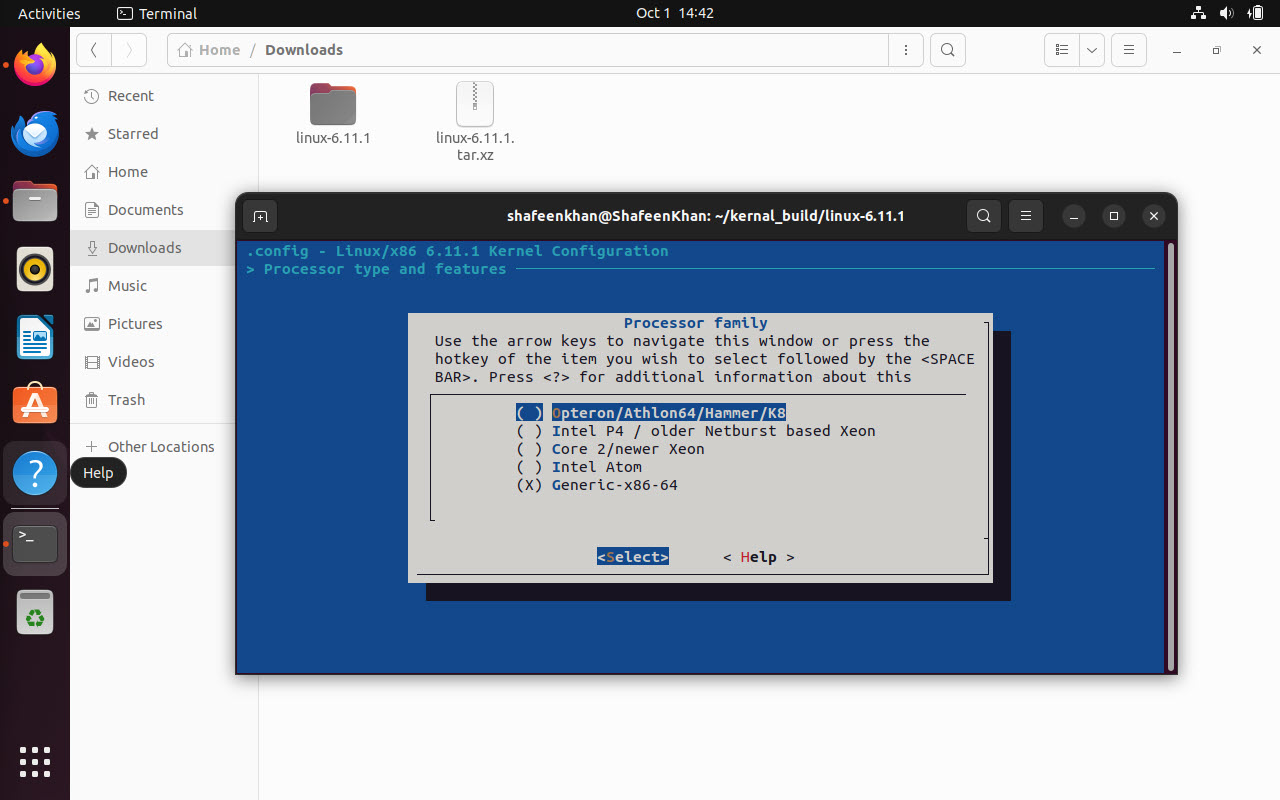
\includegraphics[width=0.8\linewidth]{58.jpg}
    \caption{Choosing a specific processor family to optimize it further.}
\end{figure}


\subsection{Kernel Configuration Setup \\- Optimizing for my own Specific Processor}
\begin{figure}[H]
    \centering
    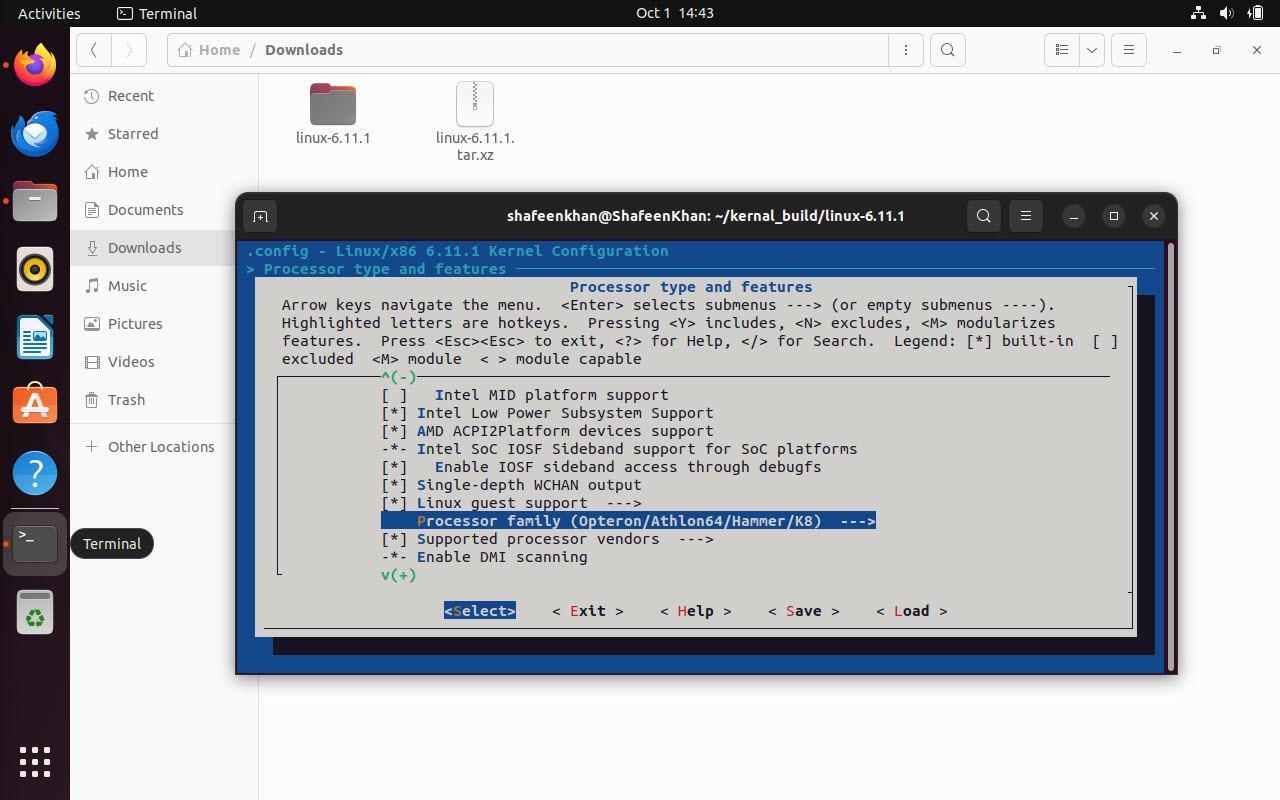
\includegraphics[width=0.8\linewidth]{57.jpg}
    \caption{As you can see i chose the Opteron version because i am using an AMD ryzen processor which will give me an edge in processing speed as it is optimized }
\end{figure}


\subsection{Kernel Configuration Setup\\ - Customize Kernel Local Version}
\begin{figure}[H]
    \centering
    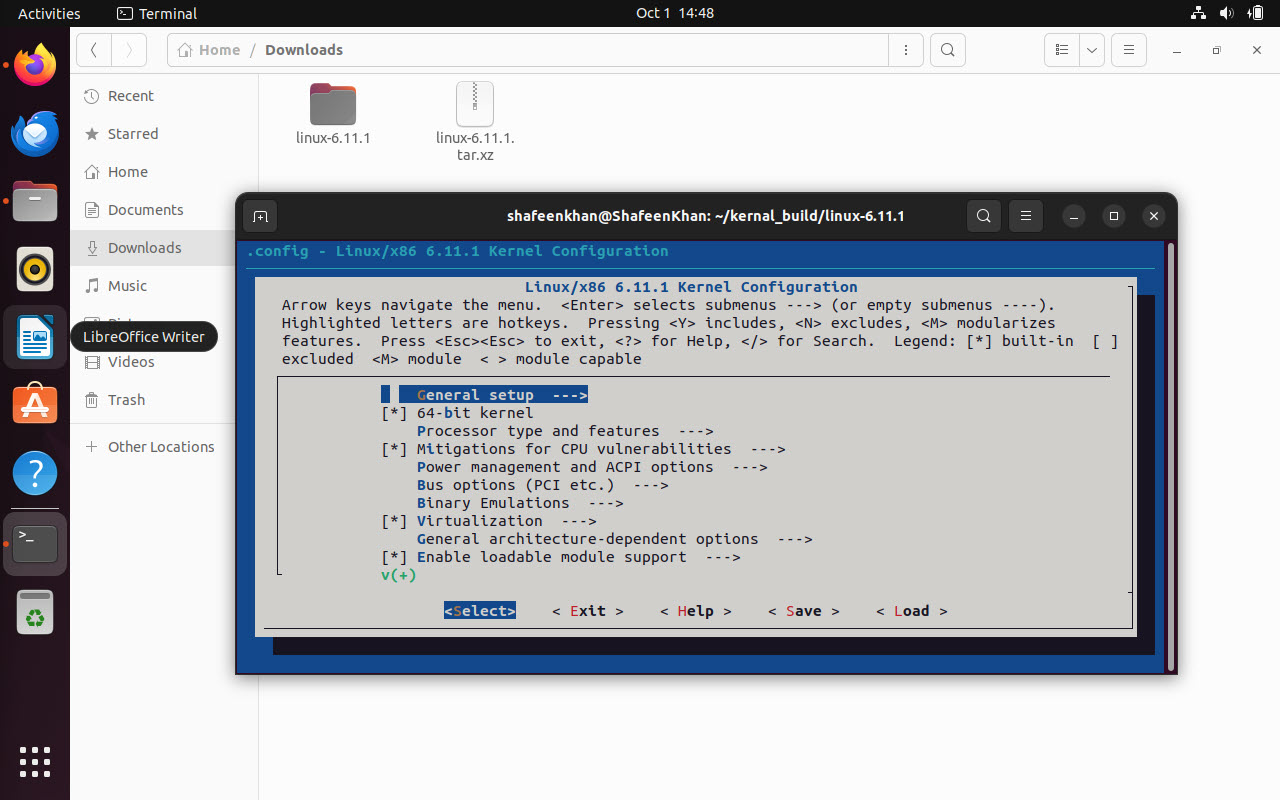
\includegraphics[width=0.8\linewidth]{56.jpg}
    \caption{Going into general setup section to change the kernal version to easily identify it}
\end{figure}

\subsection{Kernel Configuration Setup\\ - Customize Kernel Local Version}
\begin{figure}[H]
    \centering
    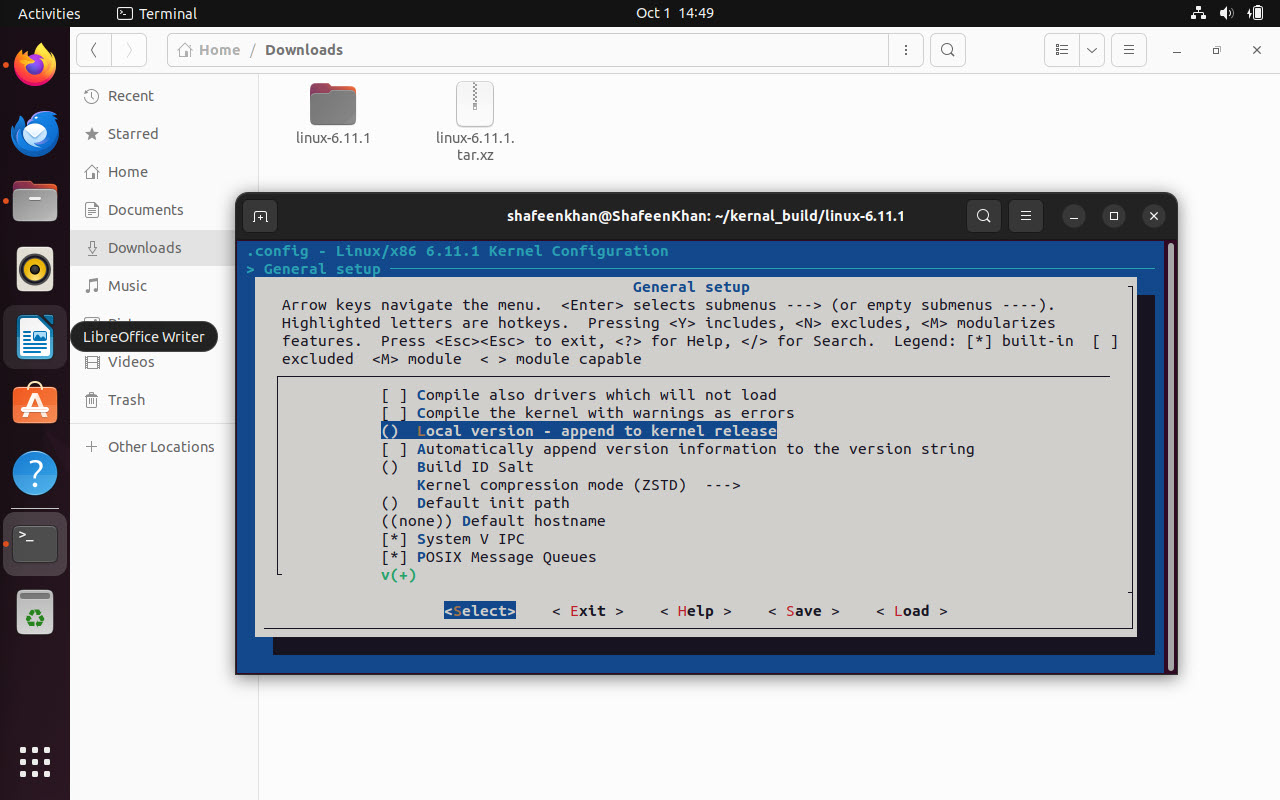
\includegraphics[width=0.8\linewidth]{55.jpg}
    \caption{Continued}
\end{figure}


\subsection{Kernel Configuration Setup\\ - Customize Kernel Local Version}
\begin{figure}[H]
    \centering
    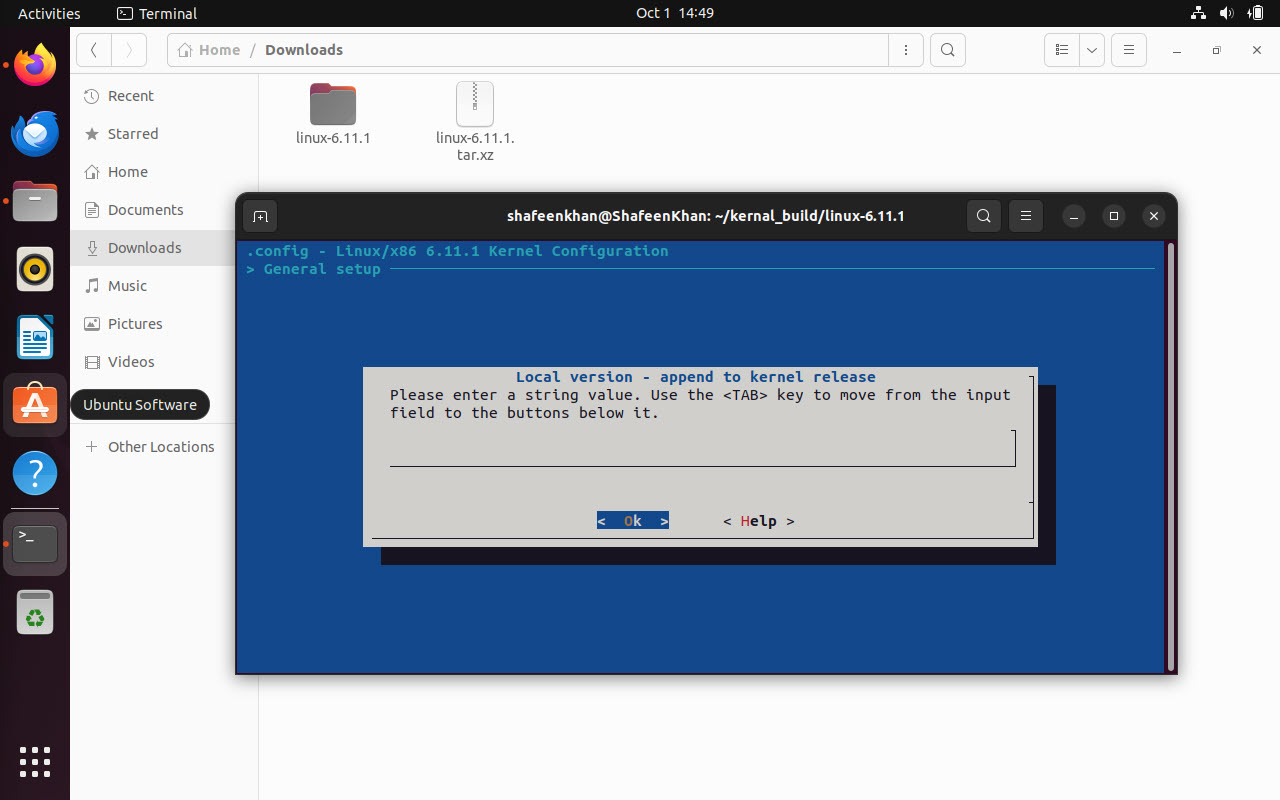
\includegraphics[width=0.8\linewidth]{54.jpg}
    \caption{Continued}
\end{figure}


\subsection{Kernel Configuration Setup\\ - Customize Kernel Local Version}
\begin{figure}[H]
    \centering
    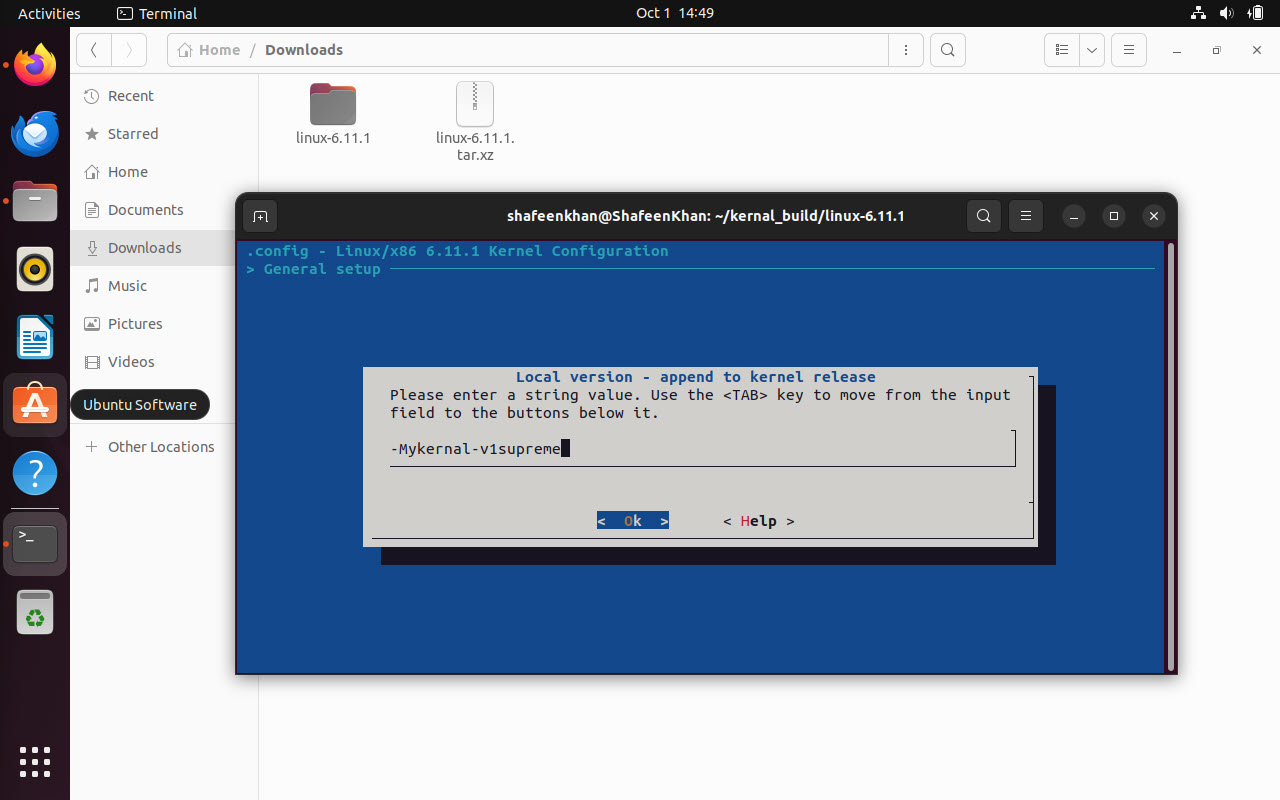
\includegraphics[width=0.8\linewidth]{53.jpg}
    \caption{Continued}
\end{figure}

\subsection{Kernel Configuration Setup\\ - Customize Kernel Local Version}
\begin{figure}[H]
    \centering
    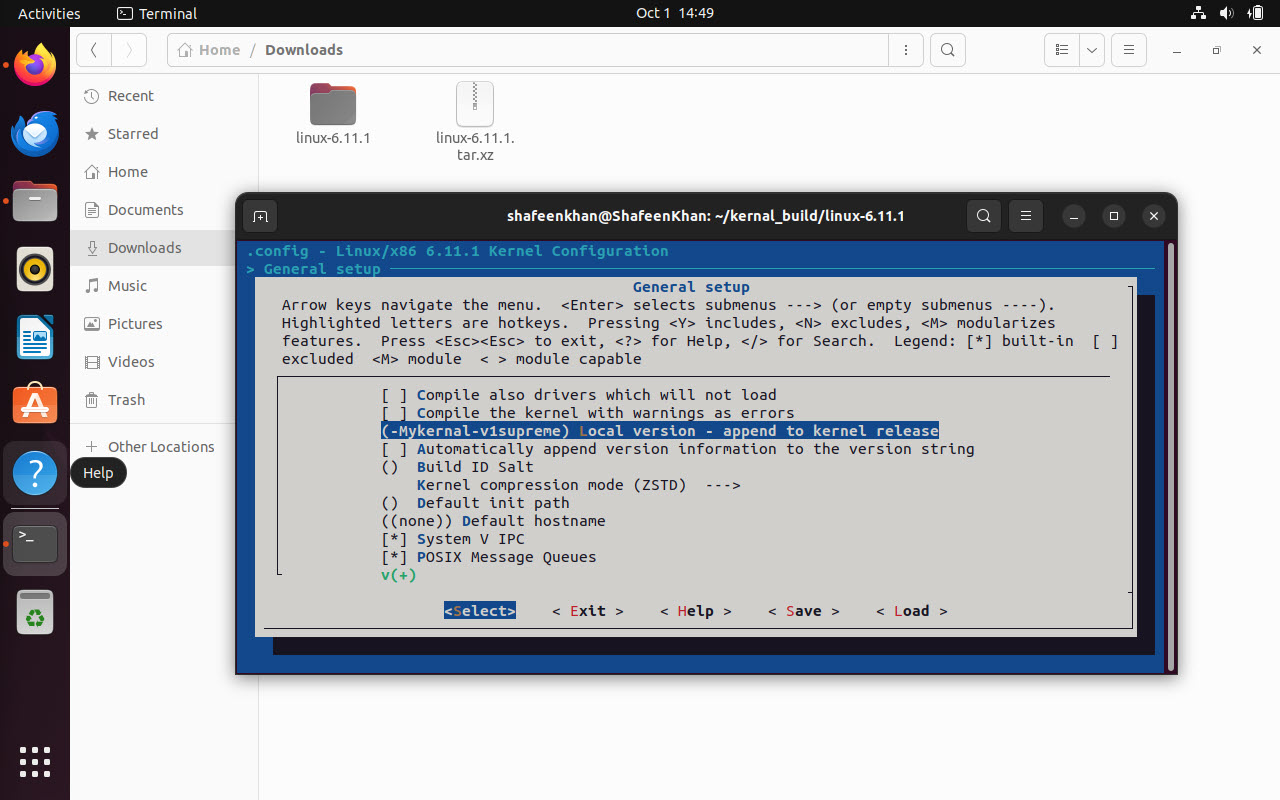
\includegraphics[width=0.8\linewidth]{52.jpg}
    \caption{Continued}
\end{figure}


\subsection{Kernel Configuration Setup \\-  Disable Unnecessary Filesystems and Drivers}
\begin{figure}[H]
    \centering
    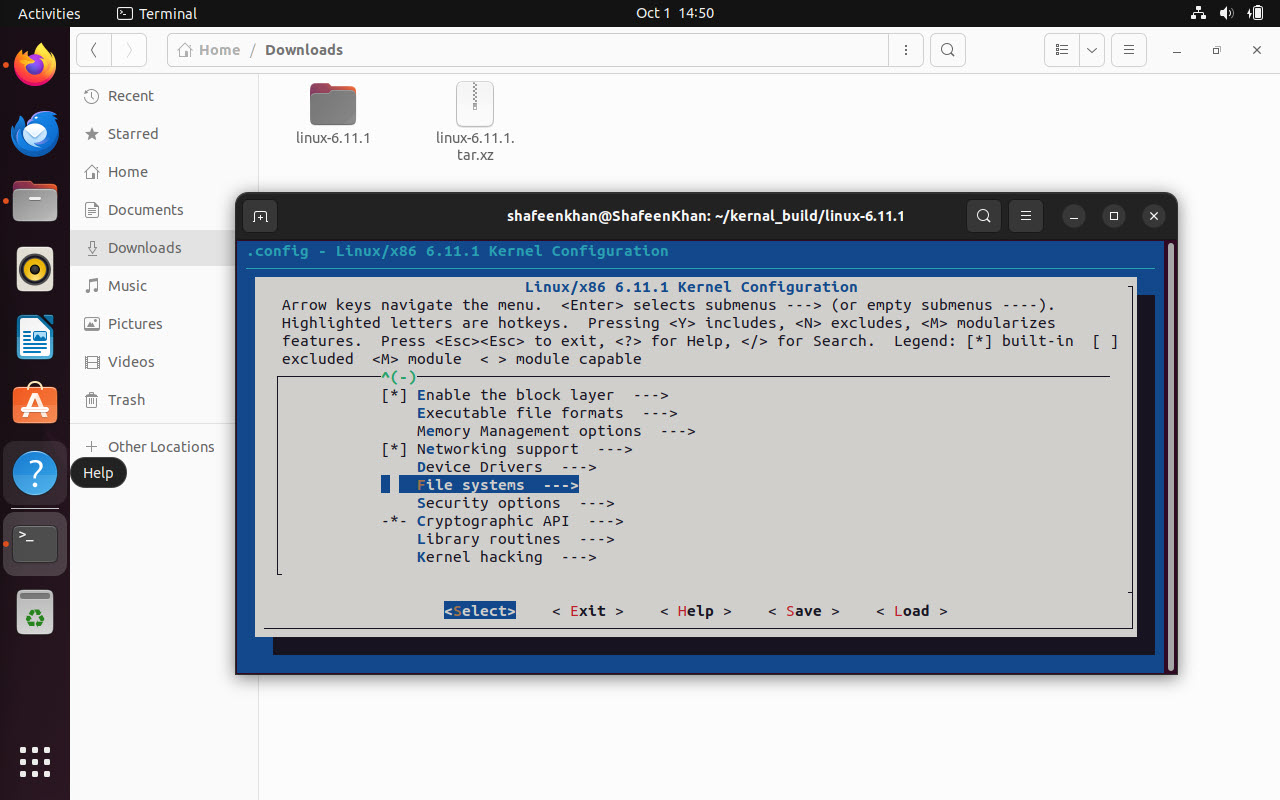
\includegraphics[width=0.8\linewidth]{51.jpg}
    \caption{Removing support for filesystems and drivers you don't use can reduce kernel size and potentially speed up boot time}
\end{figure}

\subsection{Kernel Configuration Setup \\-  Disable Unnecessary Filesystems and Drivers}
\begin{figure}[H]
    \centering
    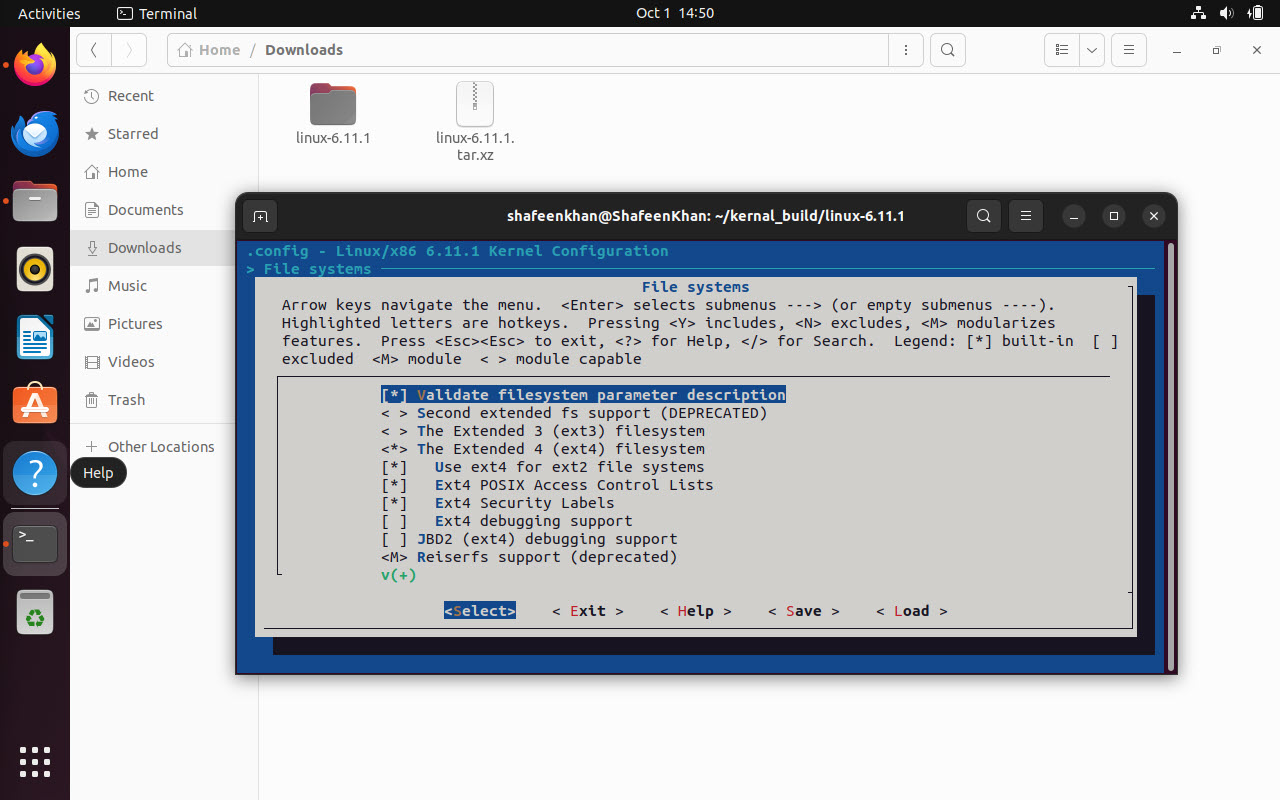
\includegraphics[width=0.8\linewidth]{50.jpg}
    \caption{Continued}
\end{figure}

\subsection{Kernel Configuration Setup \\-  Disable Unnecessary Filesystems and Drivers}
\begin{figure}[H]
    \centering
    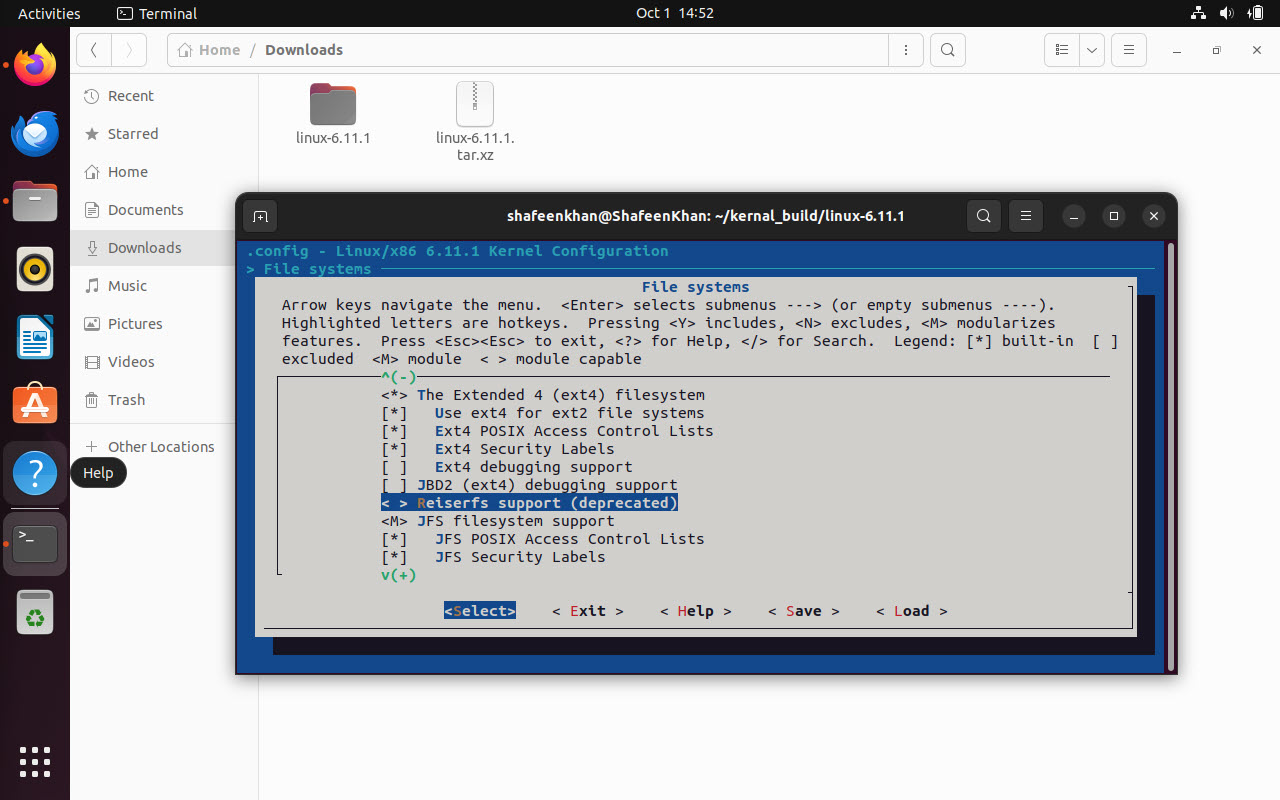
\includegraphics[width=0.8\linewidth]{49.jpg}
    \caption{Continued}
\end{figure}

\subsection{Kernel Configuration Setup \\-  Disable Unnecessary Filesystems and Drivers}
\begin{figure}[H]
    \centering
    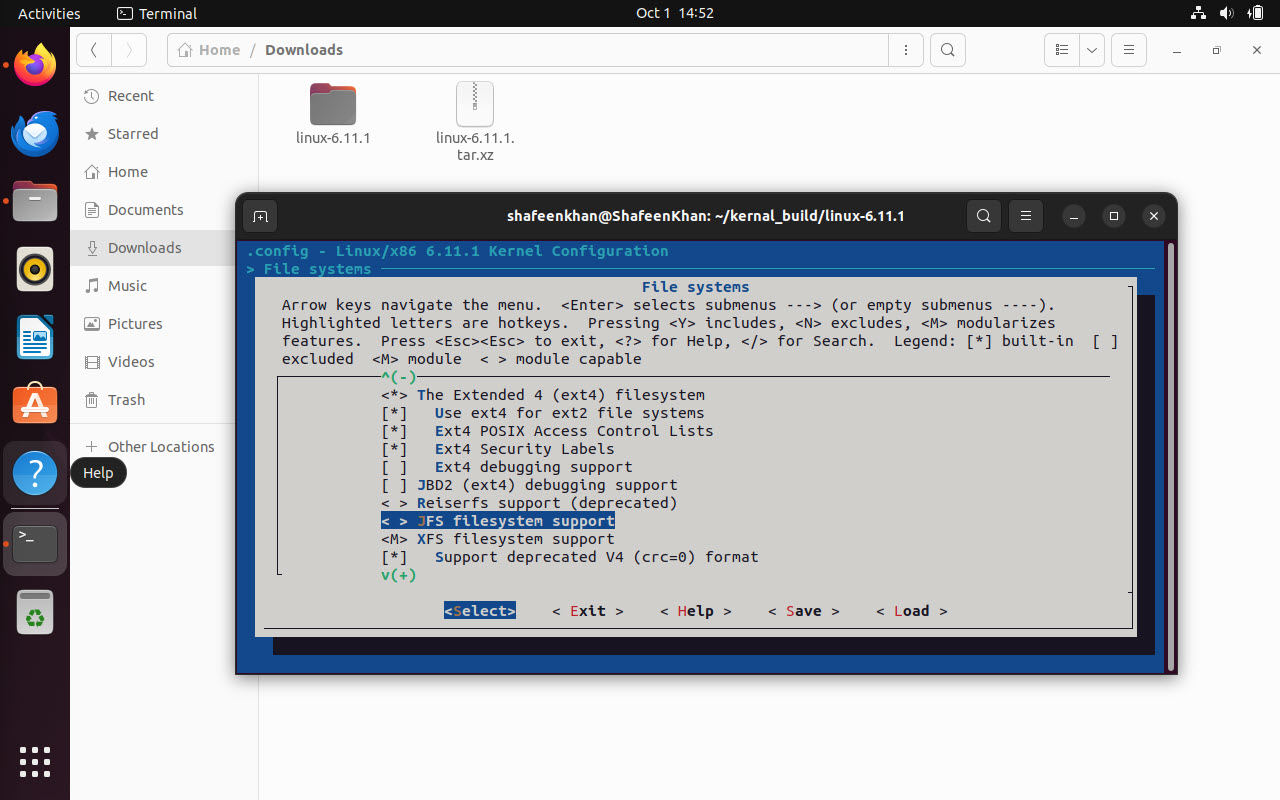
\includegraphics[width=0.8\linewidth]{48.jpg}
    \caption{Continued}
\end{figure}

\subsection{Kernel Configuration Setup \\-  Disable  RAID Controllers}
\begin{figure}[H]
    \centering
    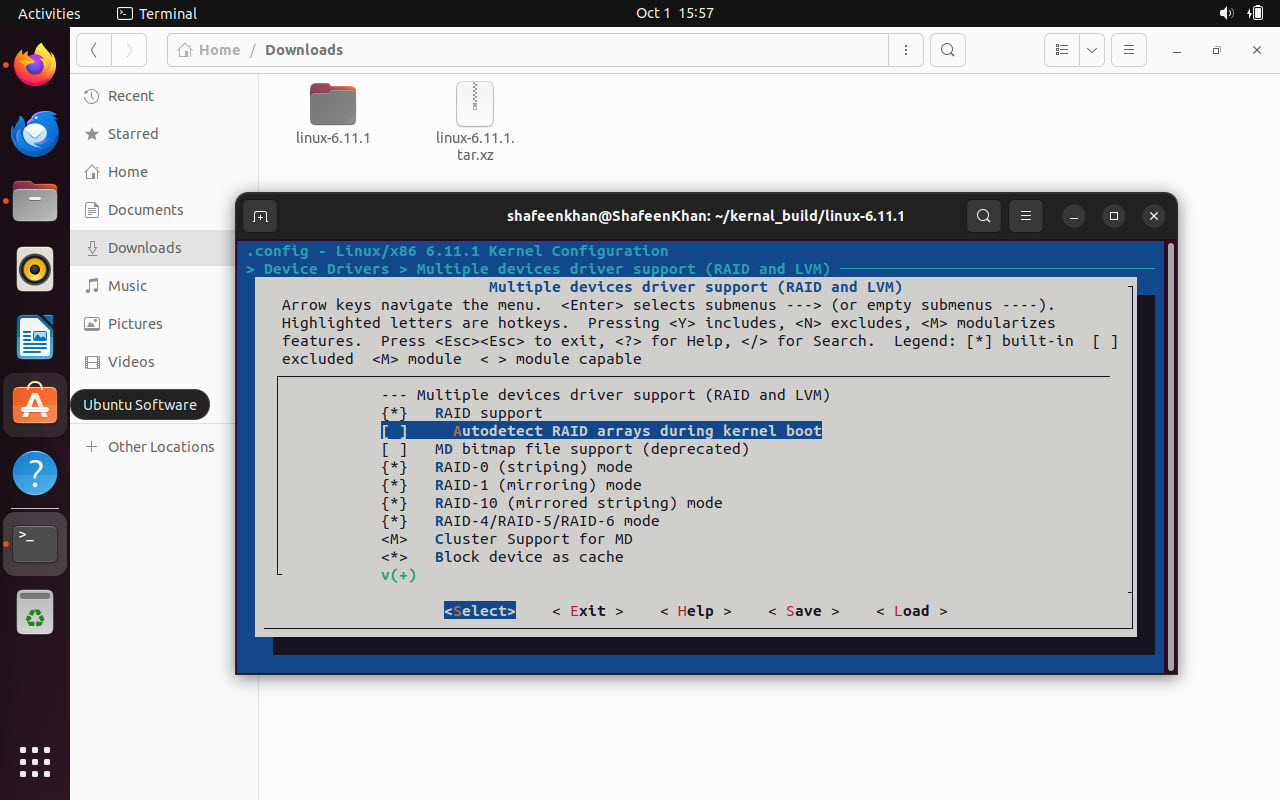
\includegraphics[width=0.8\linewidth]{45.jpg}
    \caption{Disabling unused RAID support reduces the kernel size and boot time but also minimizes security risks by removing unnecessary code}
\end{figure}

\subsection{Kernel Configuration Setup \\-  Disable  Camera}
\begin{figure}[H]
    \centering
    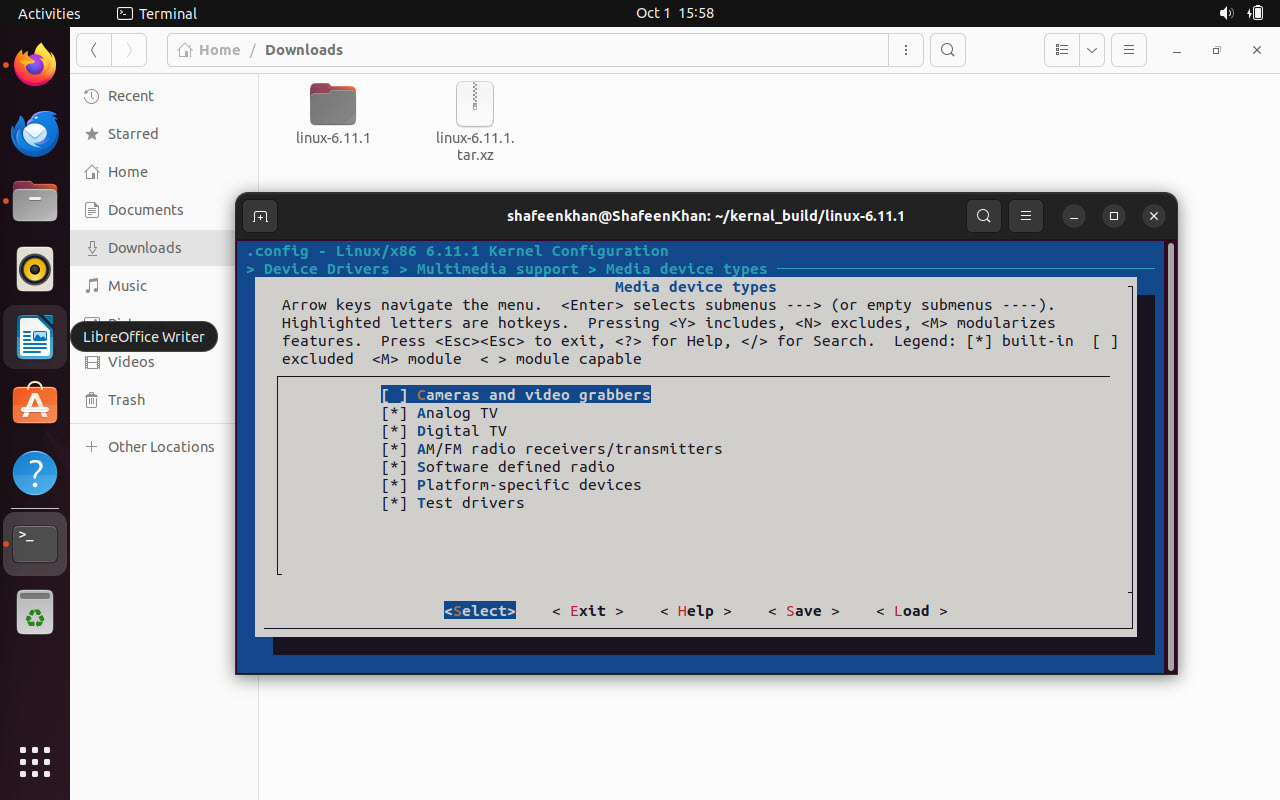
\includegraphics[width=0.8\linewidth]{44.jpg}
    \caption{Disabling camera because it is of no use , to save resources / processes and to increase security}
\end{figure}

\subsection{Enable Preemptive Kernel \\for Desktop Responsiveness}
\begin{figure}[H]
    \centering
    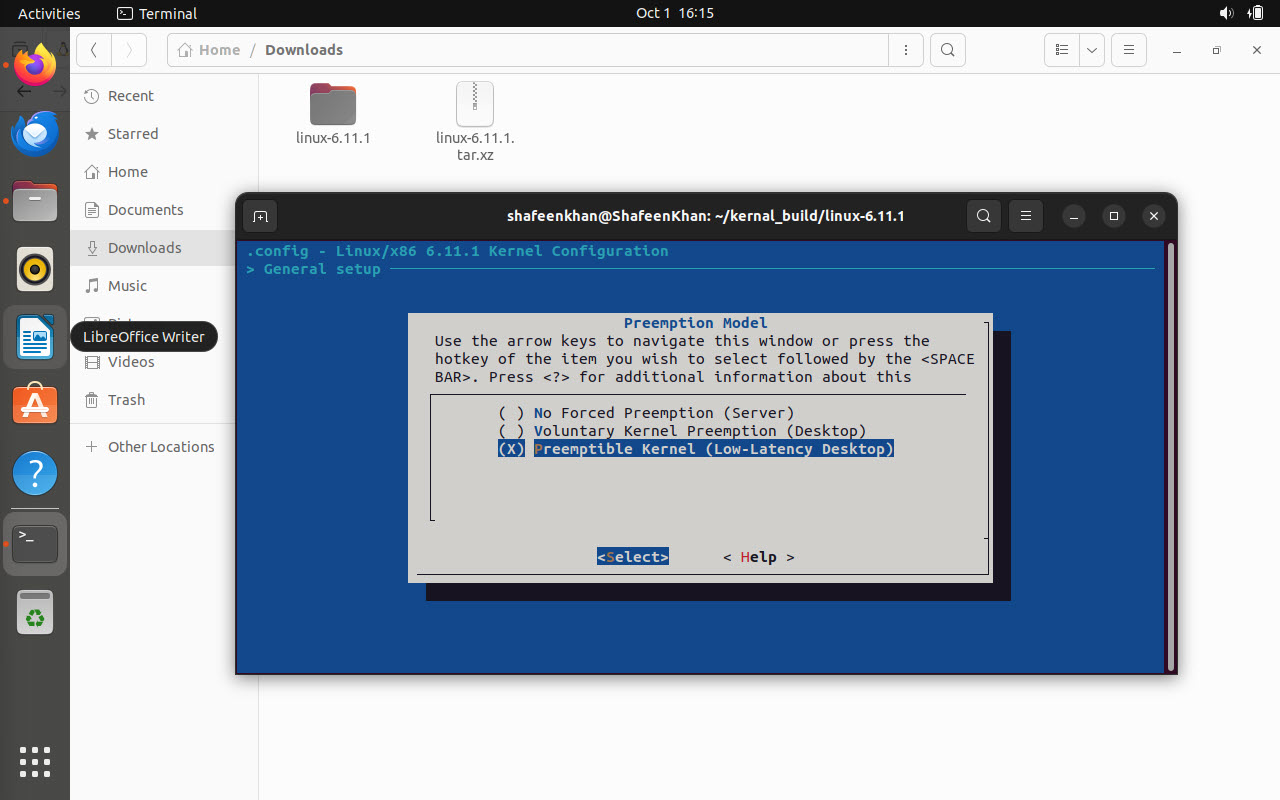
\includegraphics[width=0.8\linewidth]{38.jpg}
    \caption{A preemptive kernel allows the system to interrupt tasks more frequently, improving responsiveness in desktop environments.
}
\end{figure}

\subsection{Enable Preemptive Kernel \\for Desktop Responsiveness}
\begin{figure}[H]
    \centering
    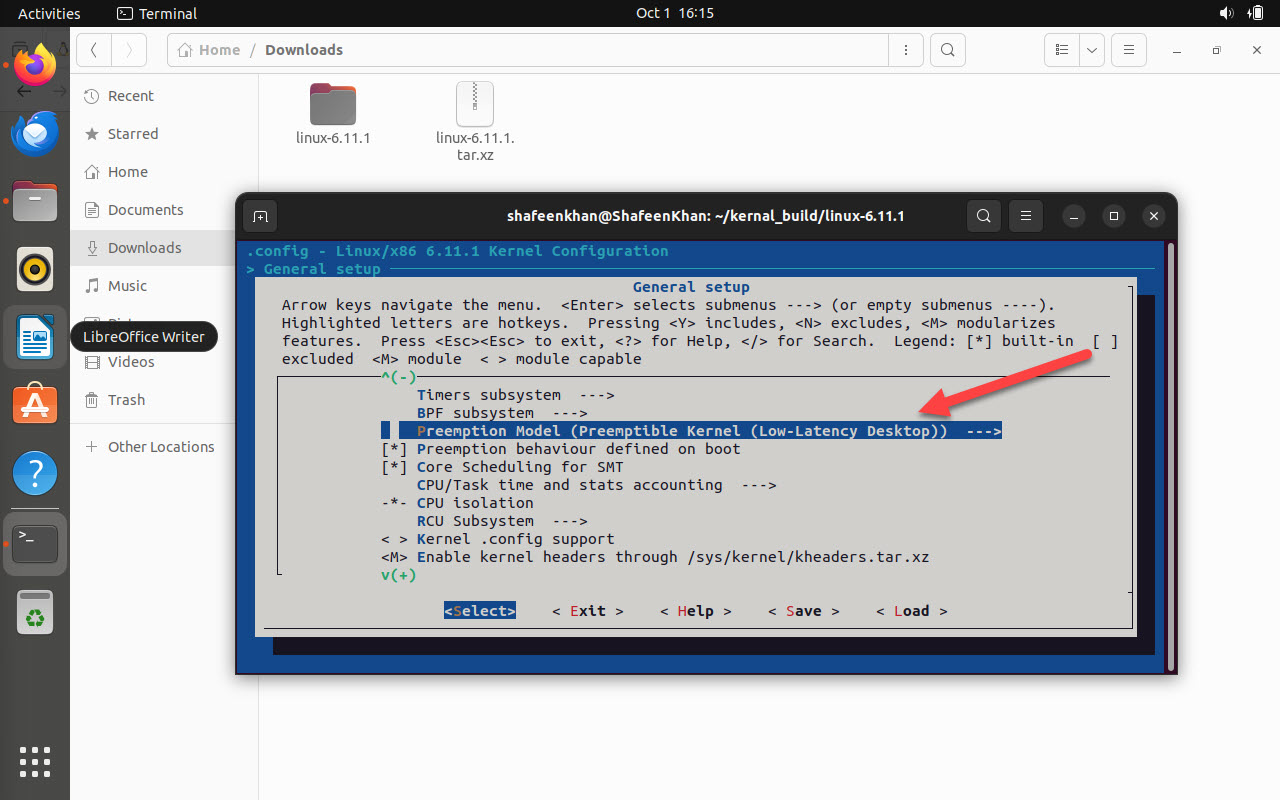
\includegraphics[width=0.8\linewidth]{36.jpg}
    \caption{continued}
\end{figure}

\subsection{Kernel Configuration Setup \\-  Save Configuration}
\begin{figure}[H]
    \centering
    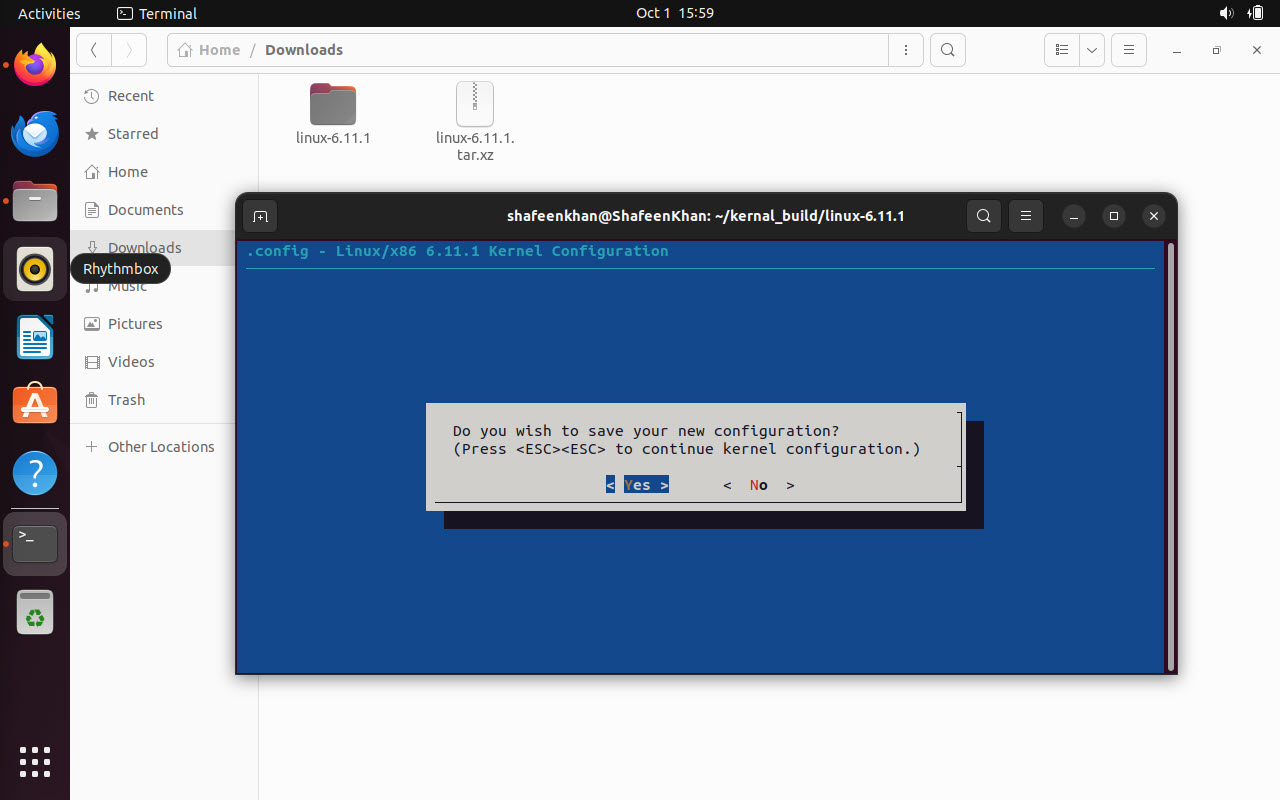
\includegraphics[width=0.8\linewidth]{43.jpg}
    \caption{}
\end{figure}

\section*{Step 8: Compiling the Kernel}
\begin{figure}[H]
    \centering
    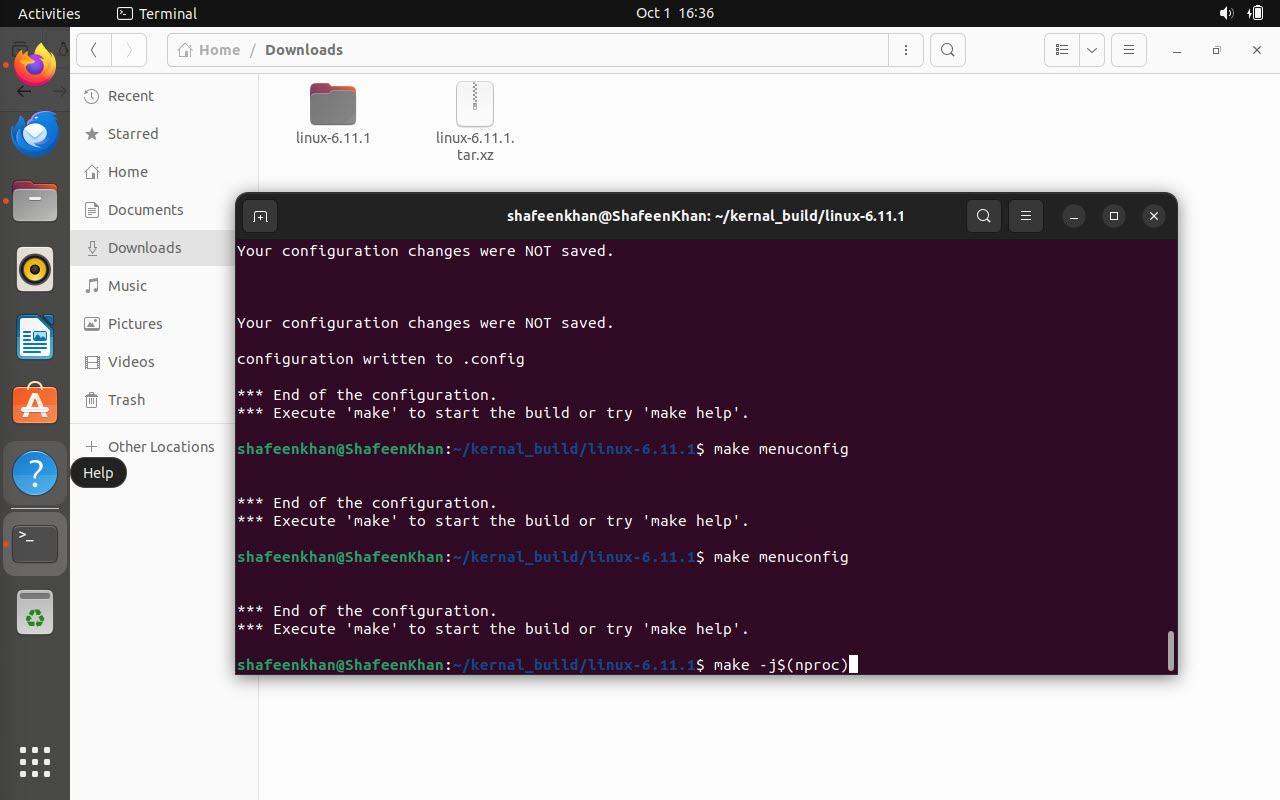
\includegraphics[width=0.8\linewidth]{26.jpg}
    \caption{Using make -j\$(nproc) , the command after make is used to utilize all cores for processing resulting in faster compilation}
\end{figure}
\subsection{Compiling the Kernel \\-  Continued}
\begin{figure}[H]
    \centering
    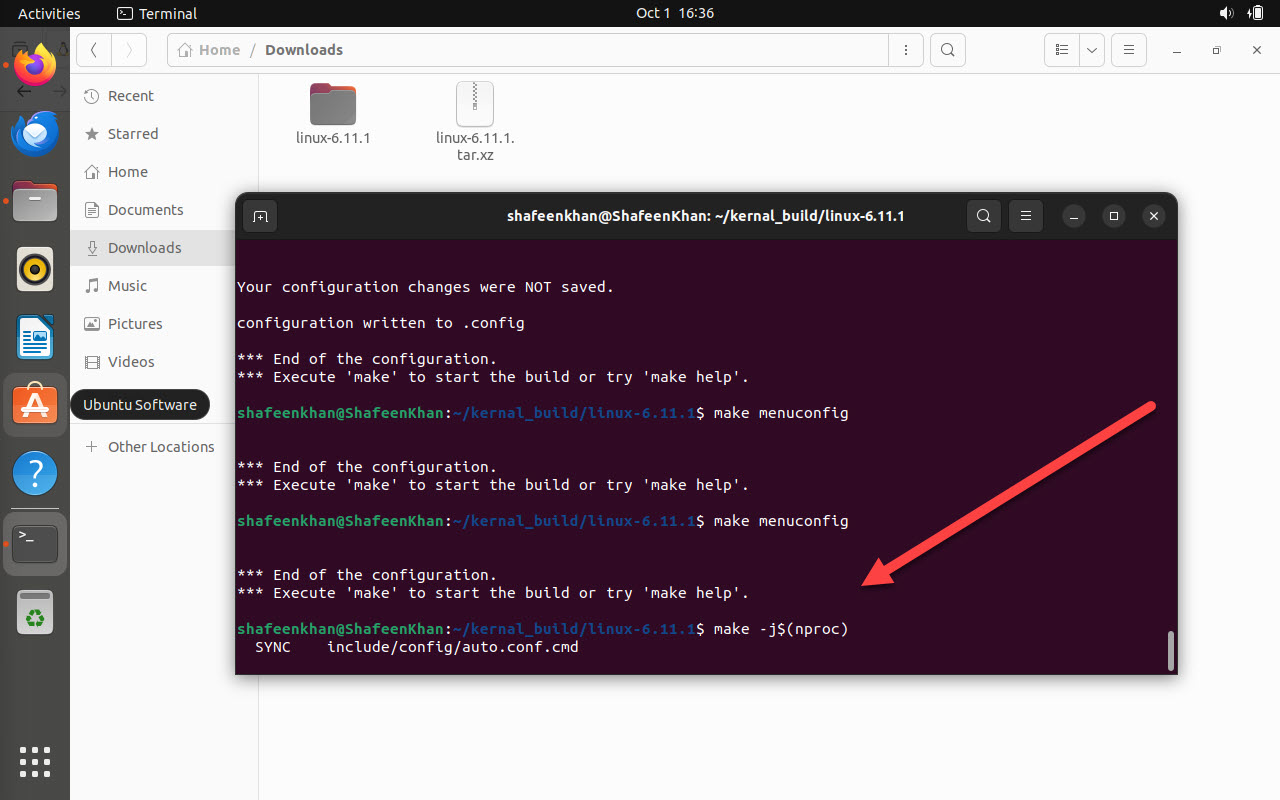
\includegraphics[width=0.8\linewidth]{25.jpg}
    \caption{}
\end{figure}


\subsection{Compiling the Kernel \\-  Continued}
\begin{figure}[H]
    \centering
    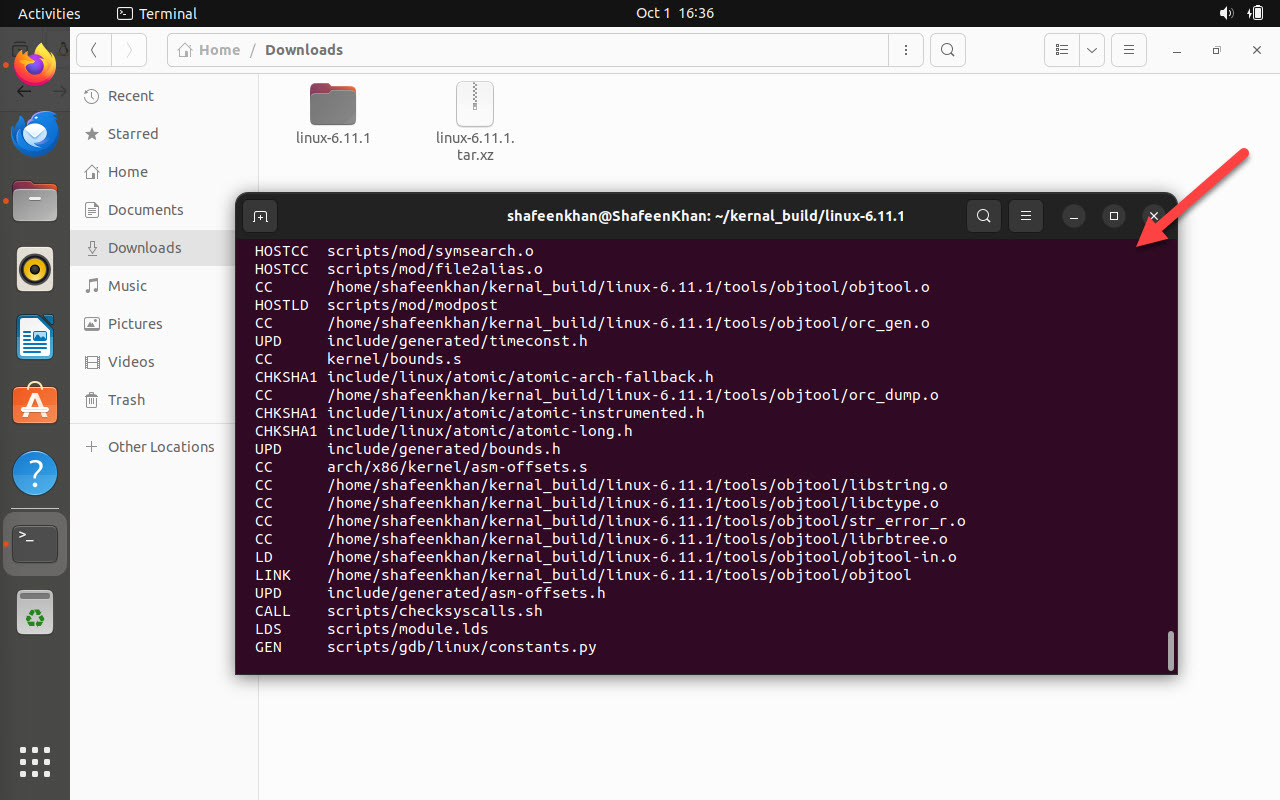
\includegraphics[width=0.8\linewidth]{24.jpg}
    \caption{}
\end{figure}


\subsection{Compiling the Kernel \\-  Continued}
\begin{figure}[H]
    \centering
    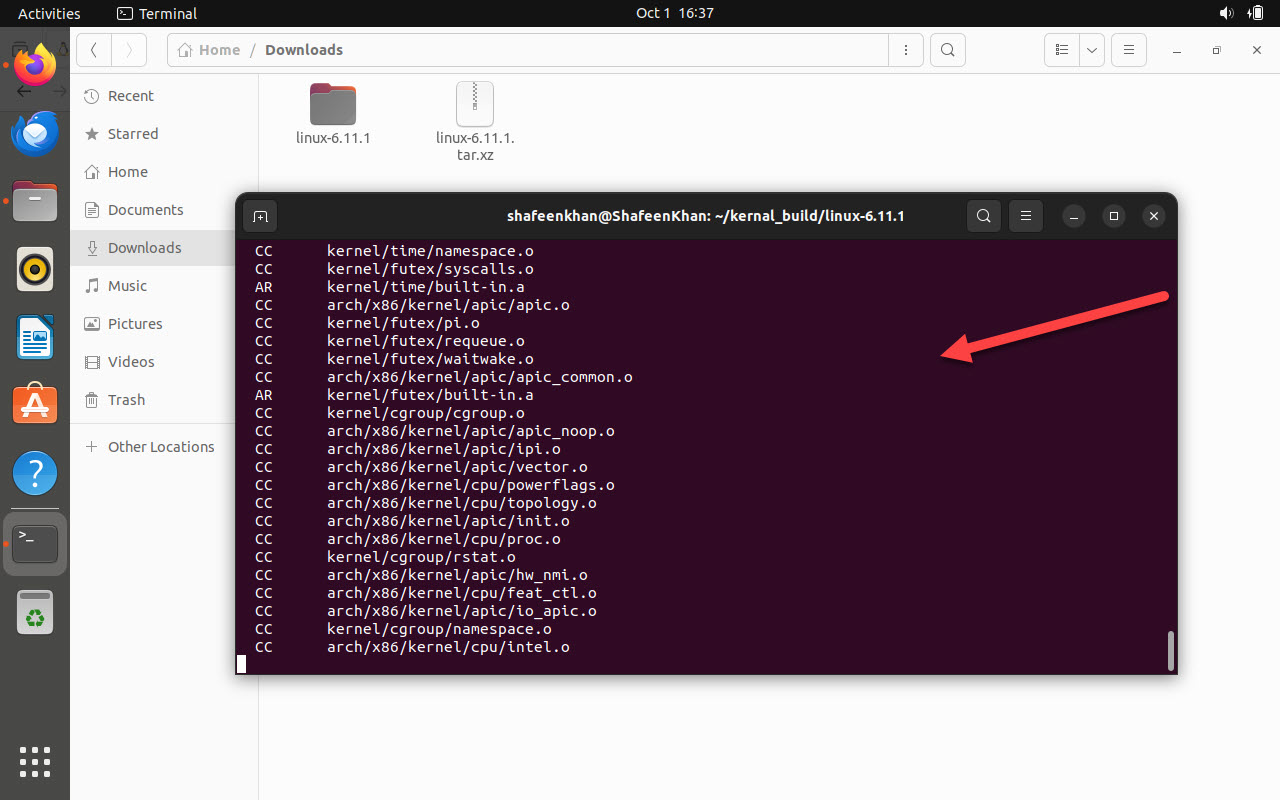
\includegraphics[width=0.8\linewidth]{23.jpg}
    \caption{}
\end{figure}


\subsection{Compiling the Kernel \\-  Continued}
\begin{figure}[H]
    \centering
    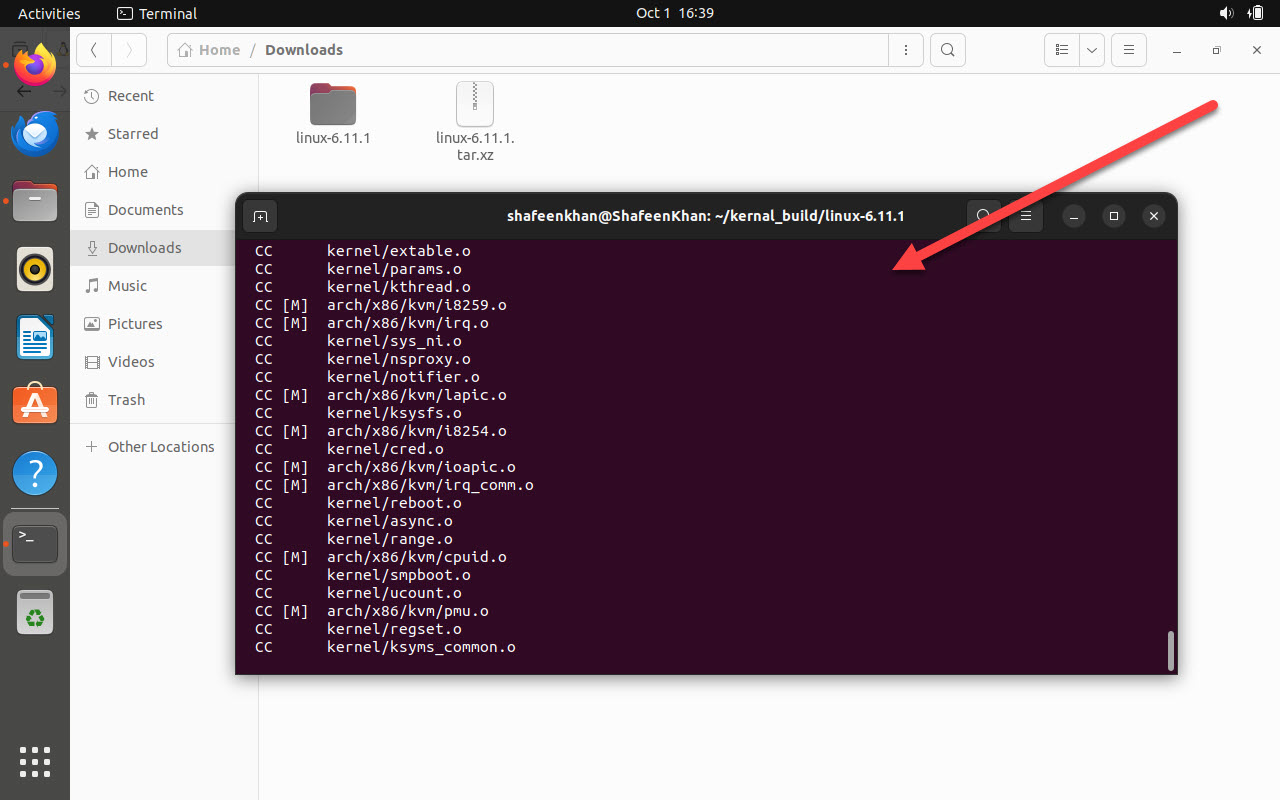
\includegraphics[width=0.8\linewidth]{22.jpg}
    \caption{}
\end{figure}


\subsection{Compiling the Kernel \\-  Continued}
\begin{figure}[H]
    \centering
    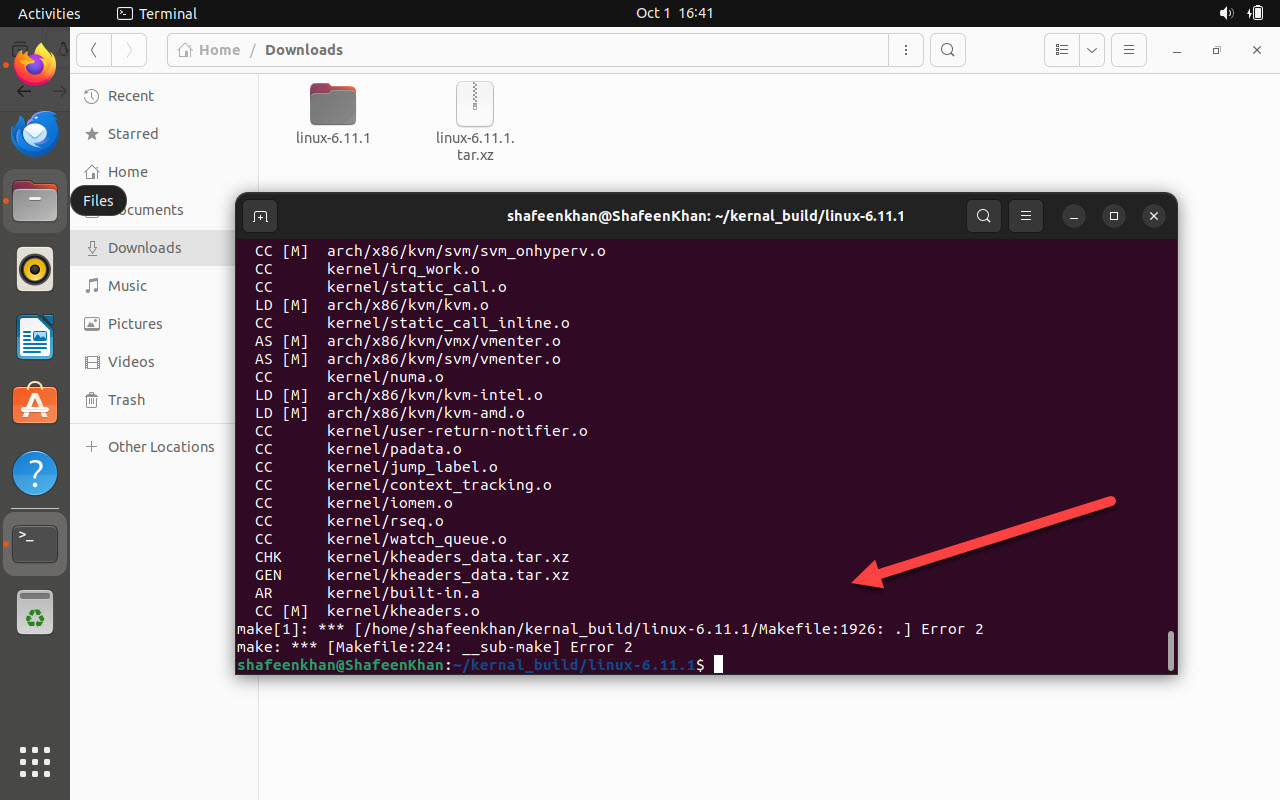
\includegraphics[width=0.8\linewidth]{21.jpg}
    \caption{it gives this error to fix this we run to commands }
\end{figure}


\section*{Step 9: ERROR WHILE - Compiling the Kernel}
This error is caused by security reasons from Linux operating system , it gives an error because installing custom linux it checks some predefined keys that are linked to your current kernal hence the keys do not match which is why it throws an error , we are gonna use some commands to disable the predefined keys and use new signatures and certifications to make the compilation possible.
" scripts/config --disable SYSTEM\_TRUSTED\_KEYS: "
" scripts/config --disable SYSTEM\_REVOCATION\_KEYS: "
These commands disable the kernel's use of trusted and revoked cryptographic keys for module and firmware verification during the build process.

\subsection{Compiling the Kernel \\-  Continued}
\begin{figure}[H]
    \centering
    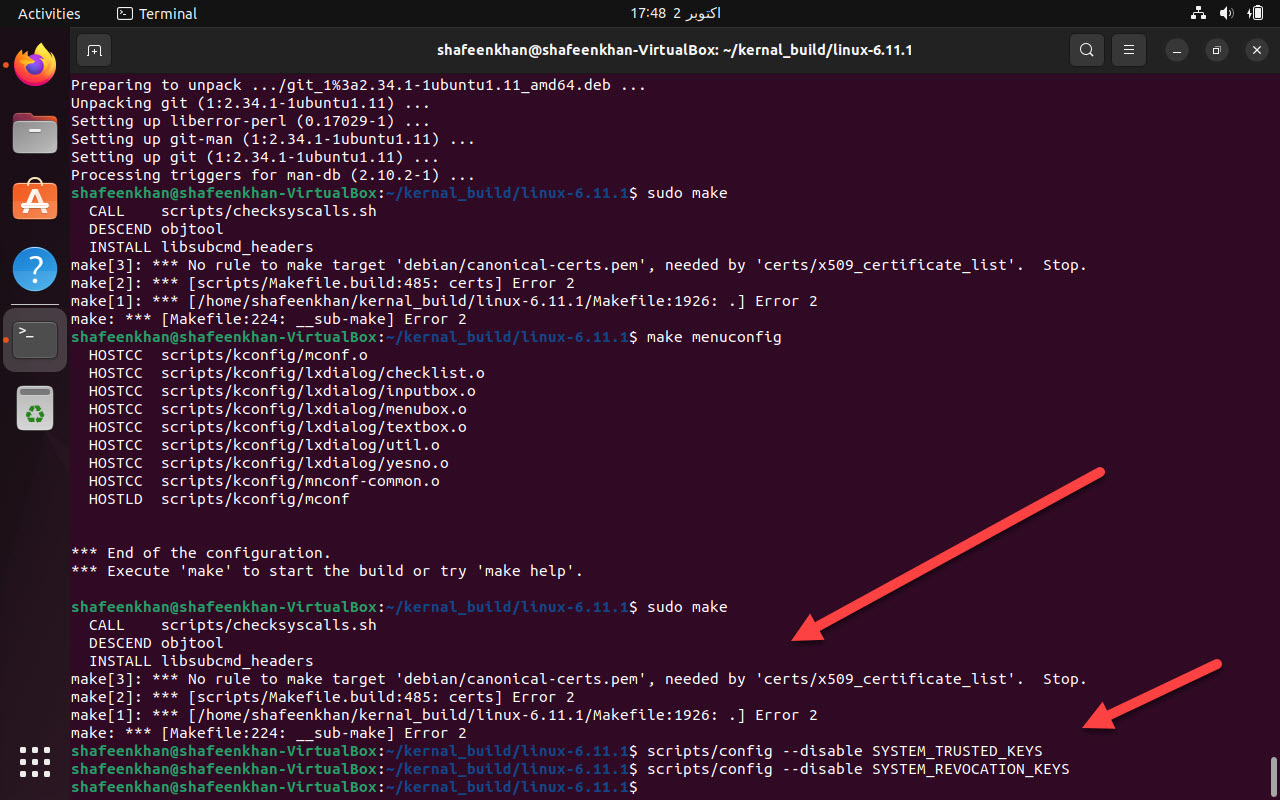
\includegraphics[width=0.8\linewidth]{19.jpg}
    \caption{The above commands fixes the errors }
\end{figure}

\section{Step 10: Installing the Kernel Modules}
\subsection{Compiling the Kernel \\-  Continued}
\begin{figure}[H]
    \centering
    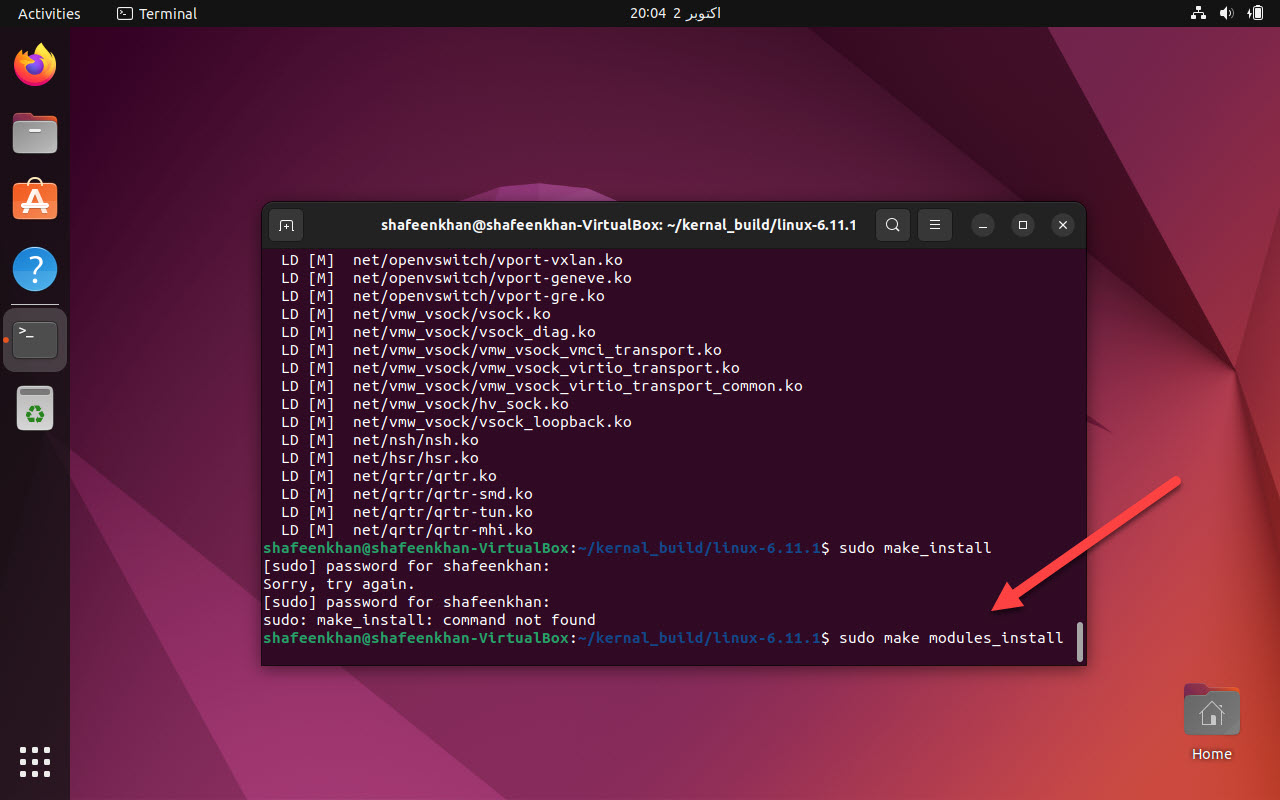
\includegraphics[width=0.8\linewidth]{14.jpg}
    \caption{This installs kernel modules to /lib/modules/<kernel-version>. }
\end{figure}

\begin{figure}[H]
    \centering
    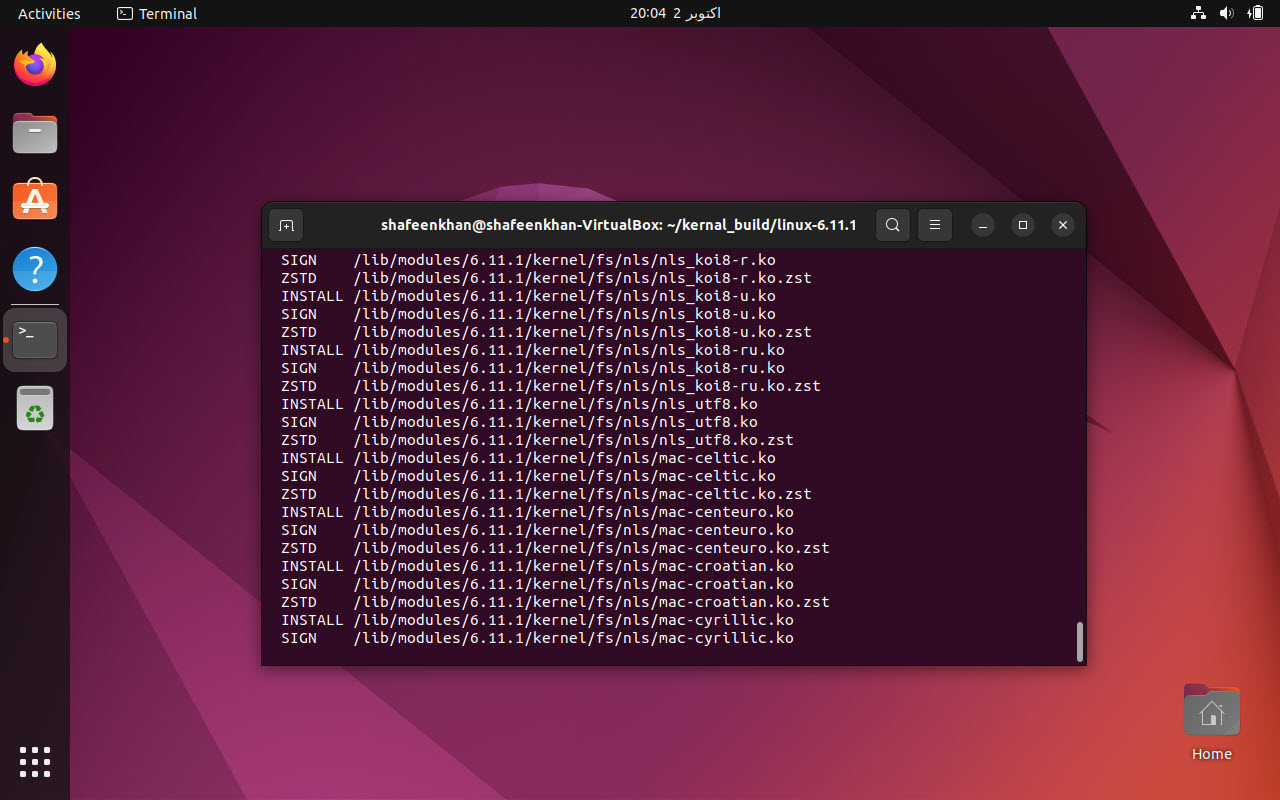
\includegraphics[width=0.8\linewidth]{13.jpg}
    \caption{ }
\end{figure}

\begin{figure}[H]
    \centering
    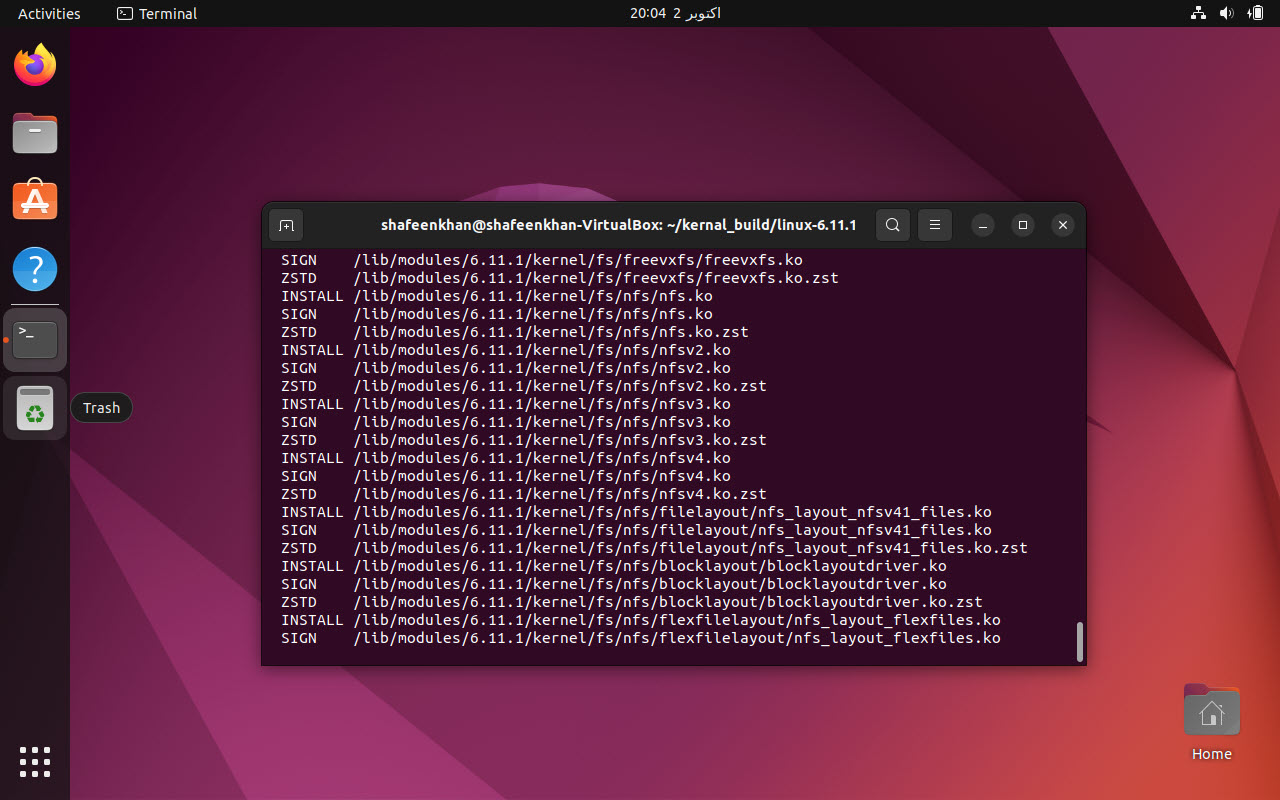
\includegraphics[width=0.8\linewidth]{12.jpg}
    \caption{ }
\end{figure}

\begin{figure}[H]
    \centering
    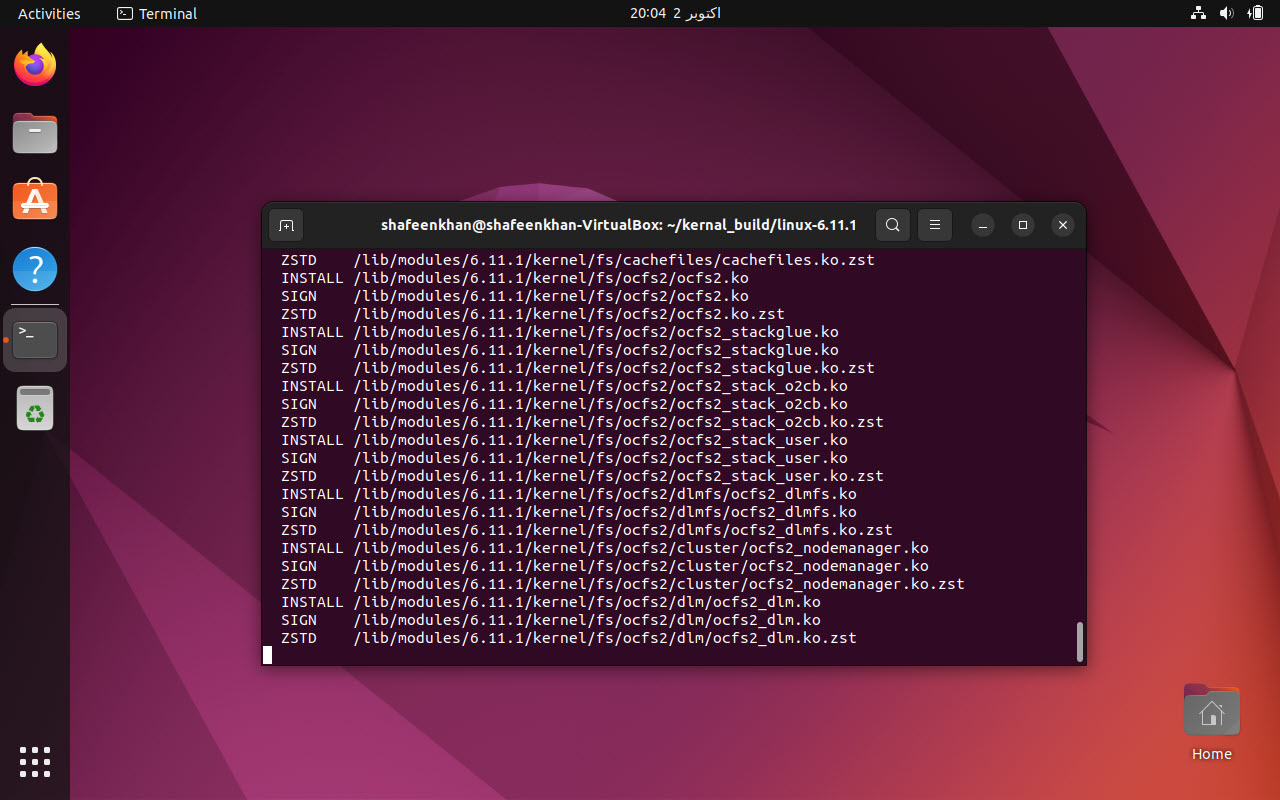
\includegraphics[width=0.8\linewidth]{11.jpg}
    \caption{ }
\end{figure}

\begin{figure}[H]
    \centering
    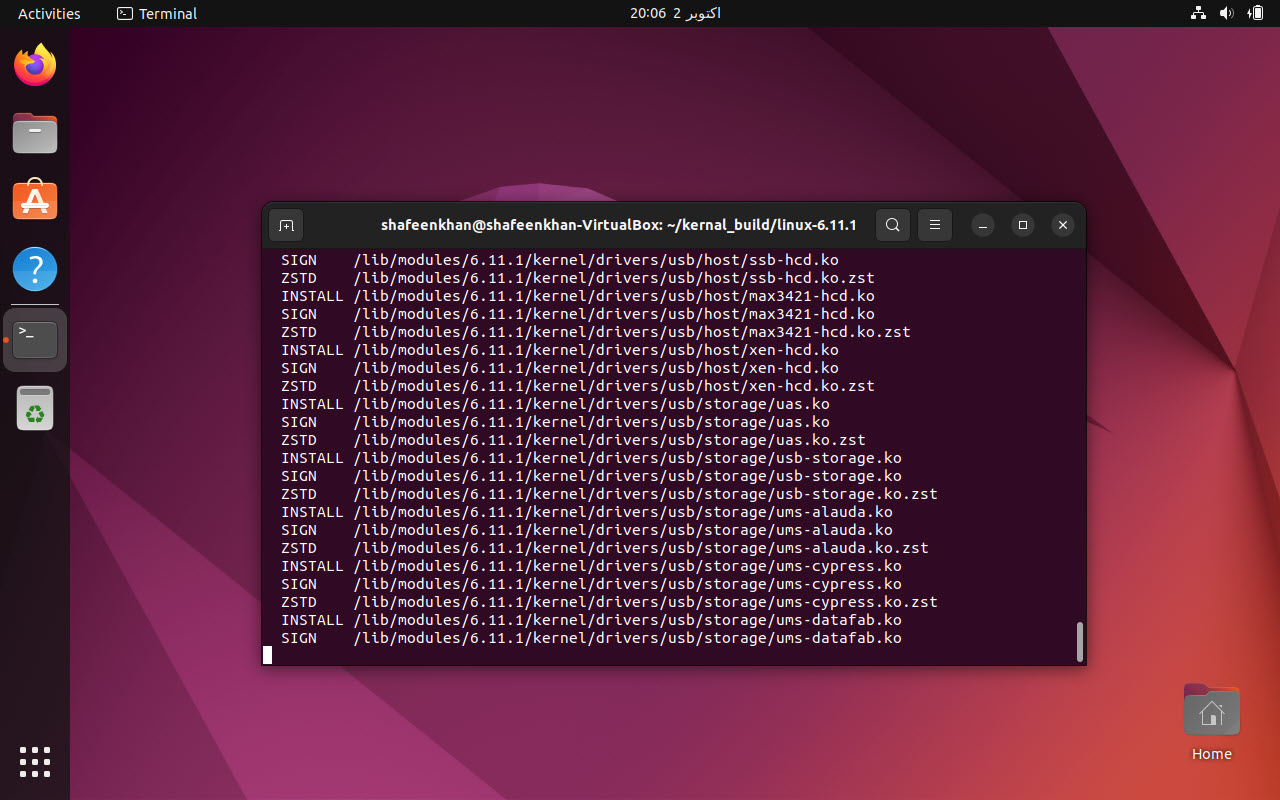
\includegraphics[width=0.8\linewidth]{10.jpg}
    \caption{ }
\end{figure}

\begin{figure}[H]
    \centering
    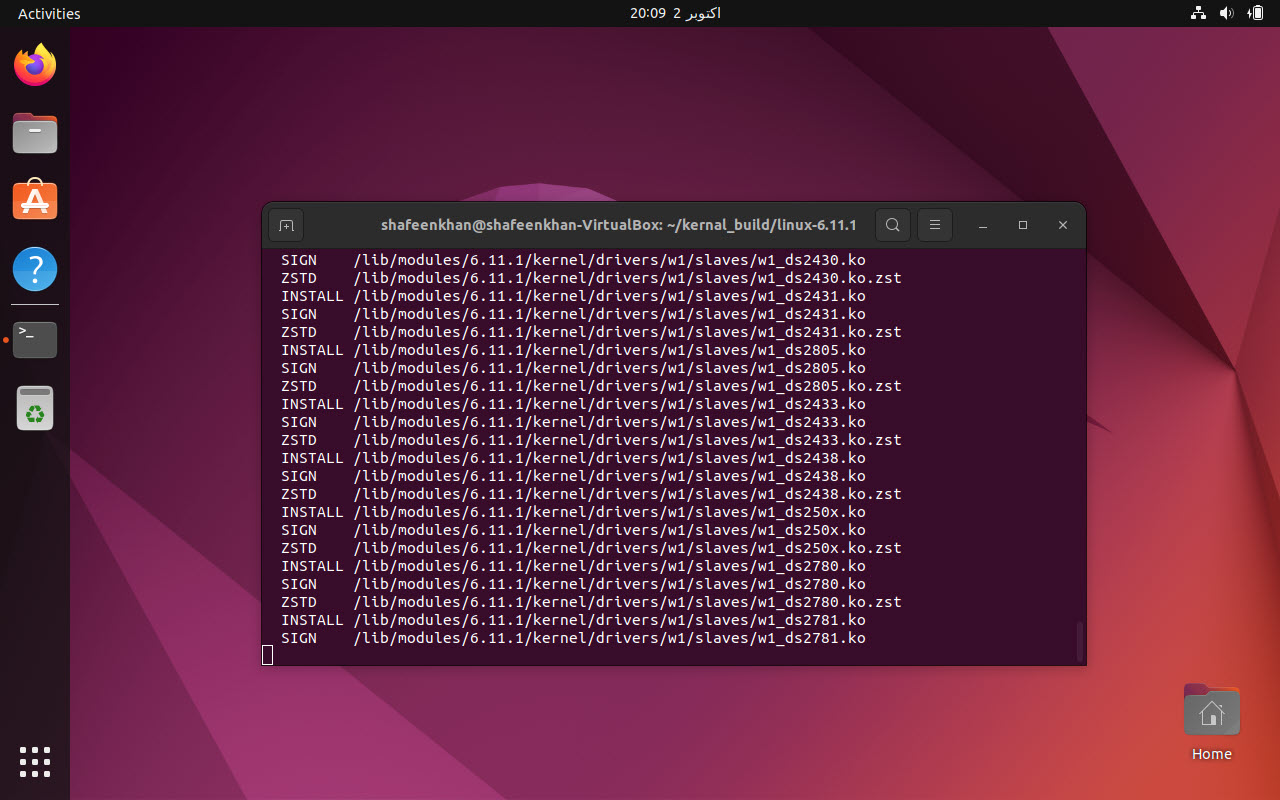
\includegraphics[width=0.8\linewidth]{09.jpg}
    \caption{ }
\end{figure}

\begin{figure}[H]
    \centering
    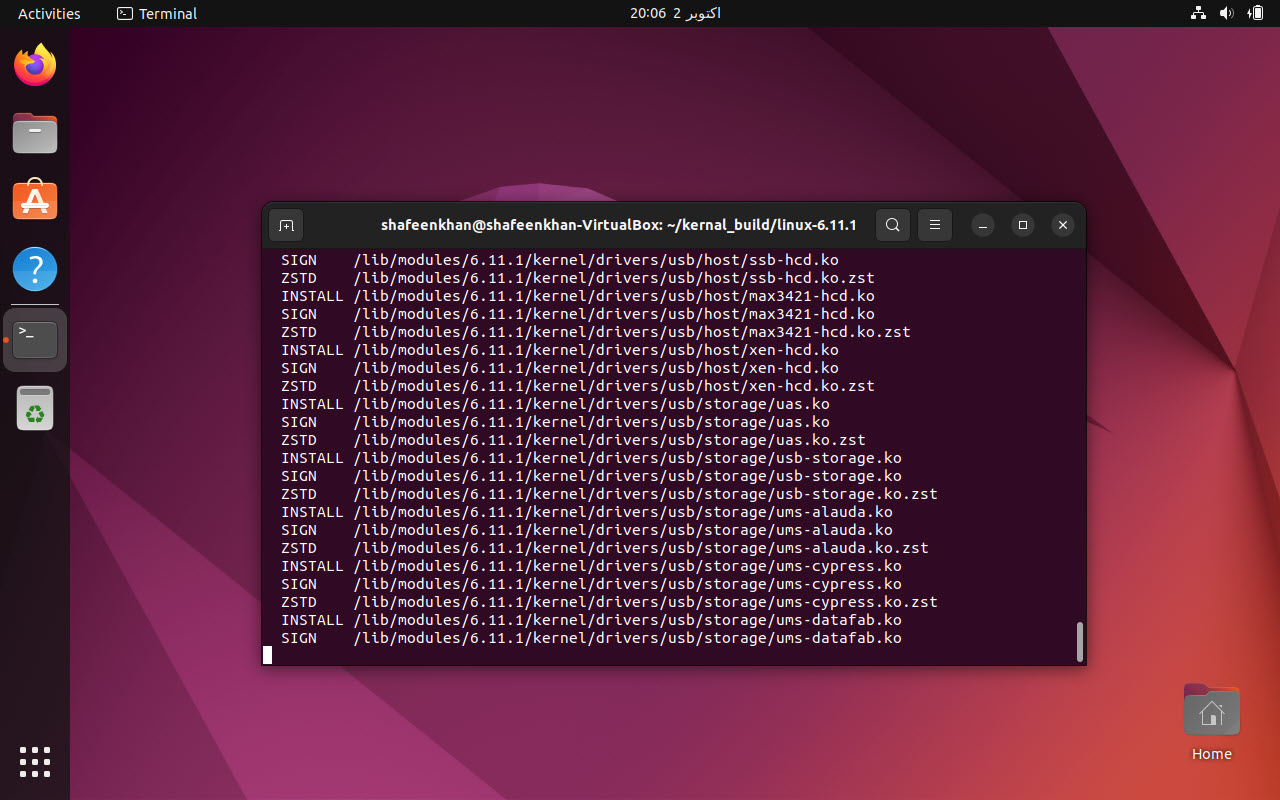
\includegraphics[width=0.8\linewidth]{10.jpg}
    \caption{Completed.}
\end{figure}


\section{Step 11: Installing the New Kernel}
\begin{figure}[H]
    \centering
    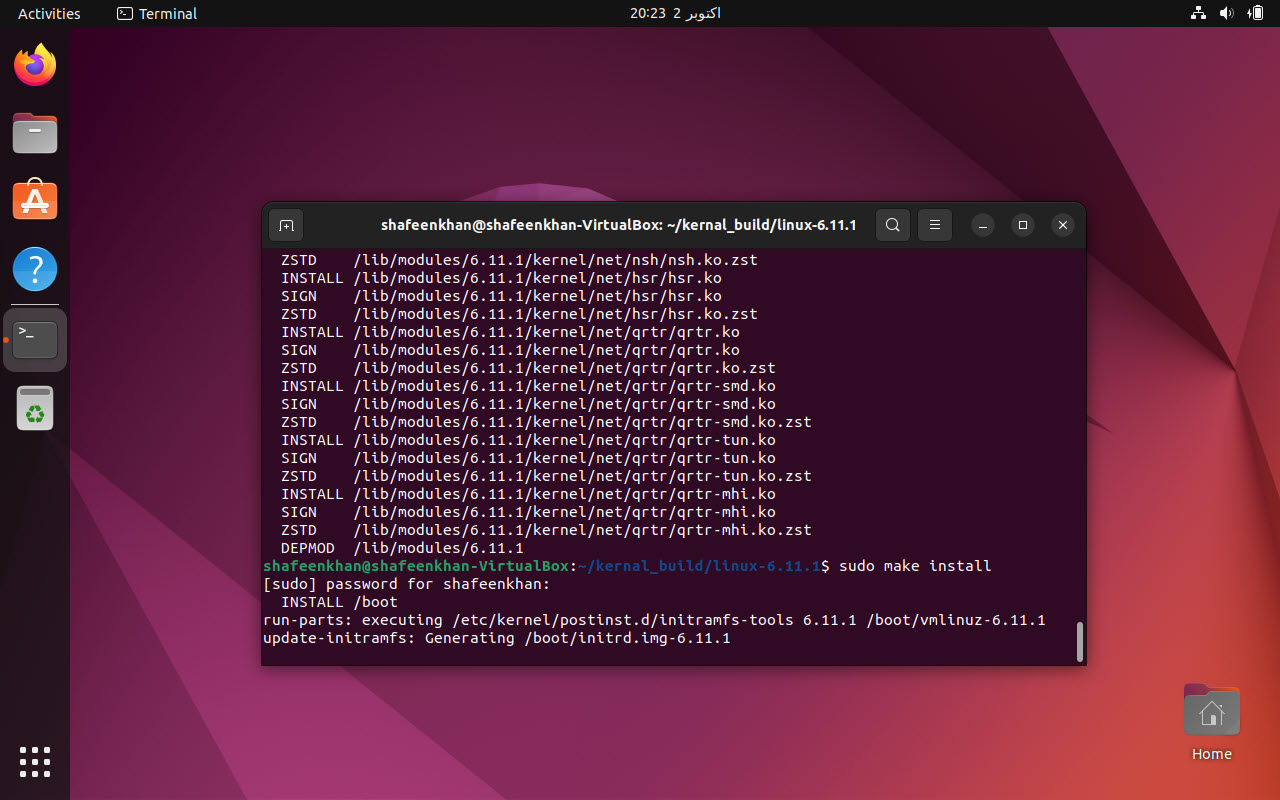
\includegraphics[width=0.8\linewidth]{06.jpg}
    \caption{This copies the kernel image (vmlinuz), system map, and config file to /boot}
\end{figure}

\begin{figure}[H]
    \centering
    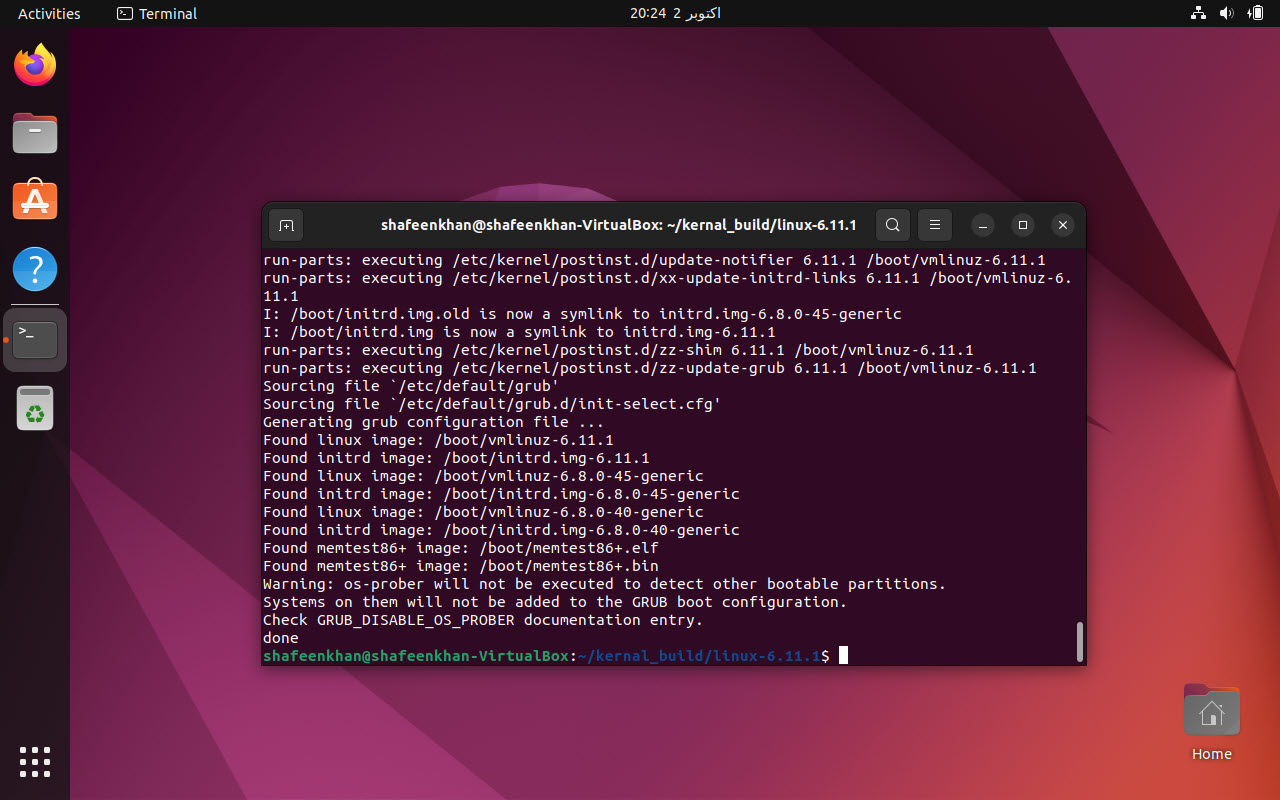
\includegraphics[width=0.8\linewidth]{05.jpg}
    \caption{Completed.}
\end{figure}

\section{Step 12: Updating the Bootloader}
\begin{figure}[H]
    \centering
    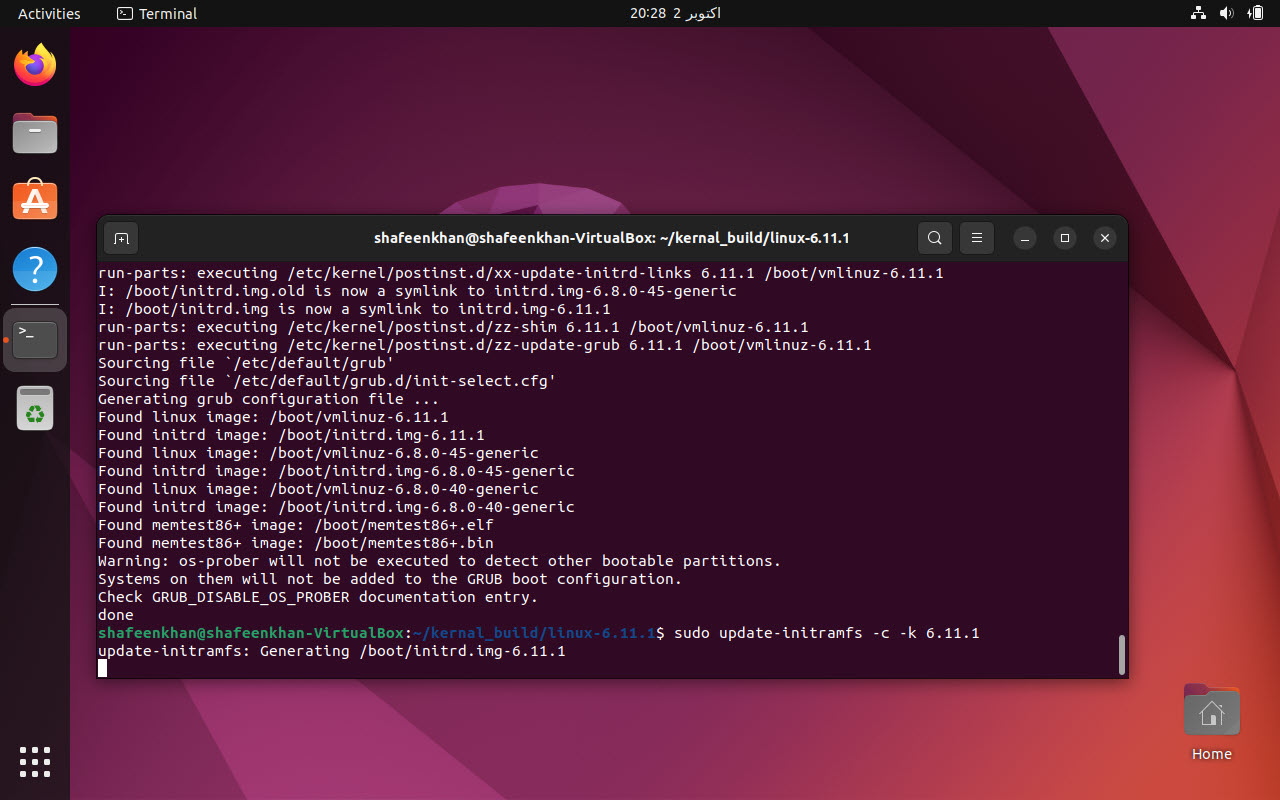
\includegraphics[width=0.8\linewidth]{03.jpg}
    \caption{update-initramfs creates a new initrd image for the new kernel.}
\end{figure}


\begin{figure}[H]
    \centering
    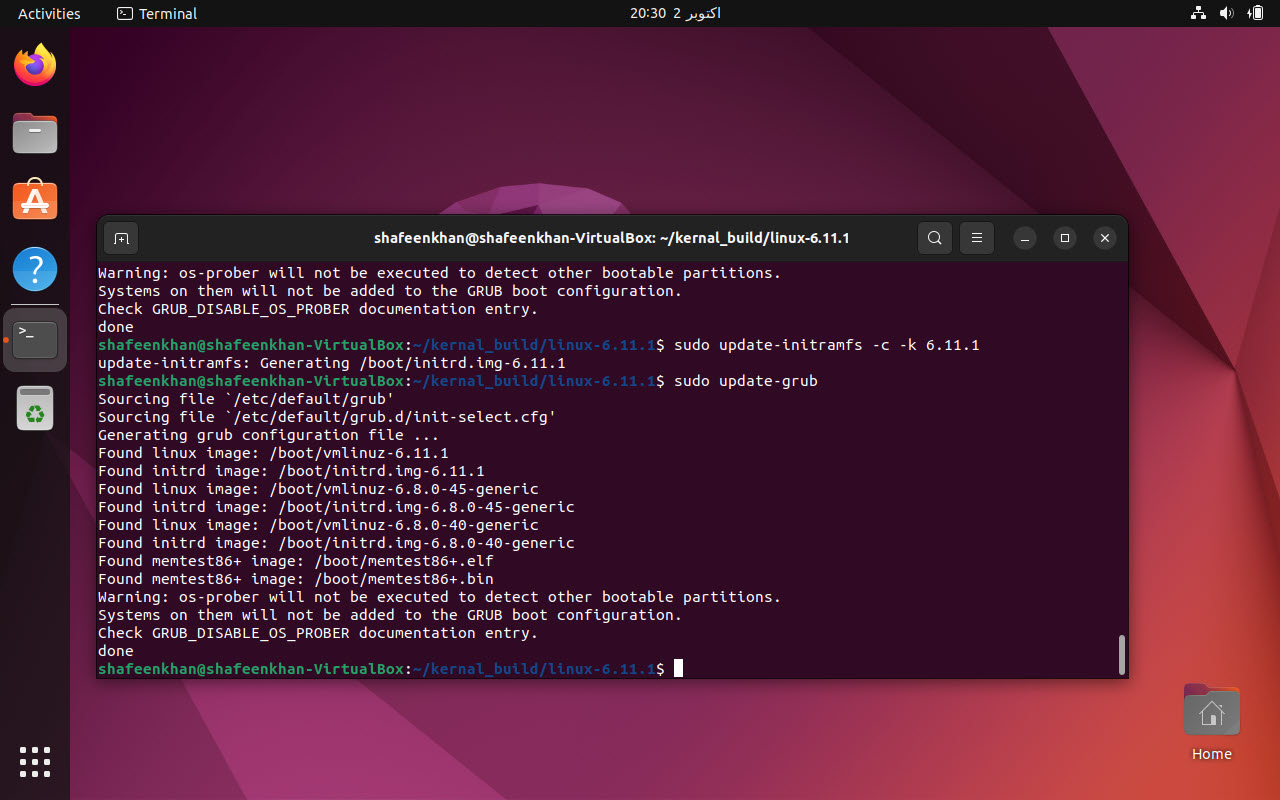
\includegraphics[width=0.8\linewidth]{01.jpg}
    \caption{update-grub scans for kernels in /boot and updates the GRUB menu.}
\end{figure}


\section{Step 13 : Step 9: Rebooting and Verify the new kernal}

\begin{figure}[H]
    \centering
    \includegraphics[width=0.8\linewidth]{00.jpg}
    \caption{uname -r to display}
\end{figure}

\section{Challanges Faced : }
One of the challenges I faced was the **kernel compilation time**. The process of running `make` took significantly longer than expected, especially since I was working in a virtual machine with limited resources. Watching it compile, I had to be patient, and it made me realize how resource-intensive this task is, even for modern systems.

Another challenge was the **kernel configuration** itself. When running `make menuconfig`, I was overwhelmed by the sheer number of options available. Deciding what to enable or disable felt like navigating a maze, and I had to be careful not to accidentally disable something critical. This added complexity made the whole process more time-consuming than I initially anticipated.
\end{document}
